\documentclass{article}
\usepackage{amsmath}
\usepackage{amssymb}
\usepackage{cite}
\usepackage[square,numbers]{natbib}
\usepackage{algorithm}
\usepackage{hyperref}
\usepackage{graphicx}
\usepackage[noend]{algpseudocode}
\usepackage[margin=1in]{geometry}
\author{Dissertation by Sean Dobson \\ Supervised by Mike Barley \& Pat Riddle \\ Dept. of Computer Science, University of Auckland \\ Bachelor of Science (Hons.) in Computer Science}
\date{\today}
\title{Predicting Search Graph Size via Domain Abstractions}
\begin{document}

\maketitle

\section{Abstract}
Determining the runtime of a search algorithm is an important problem.
In this document, we introduce Stratified Sampling with Duplicate Probabilities (SSDP),
which is an algorithm for predicting the number of nodes expanded by search algorithms
which perform Duplicate State Pruning. SSDP relies on the knowledge of
a Duplicate Probability Distribution, which gives the proportion of
nodes that are pruned when we remove duplicated states.
We show that, if we use a pure type system and a blind heuristic,
then SSDP is guaranteed to produce perfect predictions when supplied with
the correct Duplicate Probability Distribution.
We give a method of approximating this distribution which
involves performing a search in an abstracted space.
We examine the efficacy of our prediction scheme when predicting the performance
of a BFS search which solves an instance of the \(11\)-Puzzle.
Empirical analysis of the results shows that our method of prediction produces values
that are closer to the actual value than if we had simply taken the number of nodes expanded by the abstract search
as our prediction.

\section{Introduction}
In the field of Artificial Intelligence,
problem solving via State Space Search has become an area of great interest.
Some problems can readily be described in a form that implicitly defines a
graph of states. We can solve these problems via performing a search
through this state space, from the initial state to the goal state.
A number of different search techniques have been proposed \cite{dijkstra1959note, hart1968formal, korf1985depth},
but in general they each rely on the similar concept of 'expanding' states,
where we trace paths through the state space by generating the neighbours of previously generated states.
Determining the running time of these algorithms is difficult, but Barley et al. showed in 2014 \cite{barley2014overcoming}
that we could approximate this running time in terms of the number of states expanded, and the average time taken to
expand a state.
Barley et al. also observed that,
in the case of heuristic-guided searches such as A* \cite{hart1968formal},
the number of nodes expanded, and the time taken to expand a node, is highly dependent on
which heuristics are used, and how the problem is represented.
Ideally, we would like to choose our search heuristic and problem representation
so as to mimimise the running time of our search.
Unfortunately these values are difficult to predict.
Ideally, we would like some method of search runtime prediction that is much faster than running the actual search itself.
Some effort has been made toward solving this problem \cite{knuth1975estimating, purdom1978tree, chen1992heuristic, korf2001time, zahavi2010predicting, lelis2013predicting, lelis2014estimating}.
Our research aims to improve upon these efforts. \\

Specifically, we note that the majority of this research has been focused on predicting
the number of nodes expanded by Depth First Search and Iterative Deepening A* (IDA*) \cite{korf1985depth}.
IDA* does not store all of the expanded states in memory, and so it may generate the same state more than once.
Hence, these predictive methods do not apply to 'Graph Search' techniques such Breadth First Search and A*
which use Duplicate State Pruning (DSP). These search algorithms do keep all previously expanded states in memory,
and thus are able to detect duplicated states when they are generated.
The only predictive method that we are aware of which accounts for DSP is the SSDD algorithm,
as proposed by Lelis et al. in 2014 \cite{lelis2014estimating}.
In this document, we will provide an alternative predictive scheme called SSDP,
which behaves very similarly to SSDD, except for the way in which it accounts for DSP.
Specifically, we aim to first predict the proportion of nodes generated
at each depth of the search tree which will be pruned as duplicates. We refer
to these proportions as the Duplicate Probability Distribution.
This distribution is then used to inform SSDP, so that we can appropriately scale our predictions
to exclude duplicates. \\

We produce our prediction for the Duplicate Probability Distribution via a
search done on an 'abstract' version of the problem.
We automatically generate what Knoblock and Craig refer to as a 'homomorphism' \cite{knoblock1994automatically},
which maps the original unabstracted state space to a smaller abstract state space.
Problem solutions in this space are found much quicker, and so the abstract searches can be performed
very quickly. Our hope is that the abstract space still retains some of the structure of the
unabstracted space, and so we can use the duplicate probabilities in the abstract space
to predict the duplicate probabilities in the real space. To that end,
we provide a method of mapping the abstract duplicate probability distribution to a prediction
for the unabstracted duplicate probability distribution. \\

We have constrained the scope of our research to the problem of predicting the number of nodes expanded
by DSP Breadth First Search. We are not using heuristics,
so this allows us to effectively eliminate the need to account for
the time spent computing heuristic values. Our predictions for the running time
will be expressed solely in terms of the number of nodes expanded.
Korf et al. observed in 2001 \cite{korf2001time} that when running A* with a heuristic \(\hat{h}\),
the search will expand all nodes \(n\) with \(g(n) + \hat{h}(n) \leq h(s_0)\),
where \(g(n)\) is the cost to reach \(n\) from the initial state \(s_0\),
\(\hat{h}(n)\) is the heuristic value for \(n\), and \(h(s_0)\) is cost to reach the goal state from \(s_0\).
Hence, when trying to predict the number of nodes expanded by A*,
we must account for the extra pruning effects produced by the heuristic.
So by limiting ourselves to just considering the nodes expanded by DSP BFS,
we can simplify our predictions by ignoring the effects of heuristics. \\

In terms of testing the viability of our approach,
the analysis and experimentation that we perform is specific to the Sliding-Tile Puzzle problem domain.
This is was the same problem domain that Korf et al. used in 2001 \cite{korf2001time} to test
their predictive scheme.
We have chosen this domain because its state space exhibits a predictable structure.
Edelkamp et al. refer to these as kinds of domains as 'regular' \cite{edelkamp1998branching}.
They showed that the branching factors for these regular domains (i.e. the out-degrees of the states)
can be characterised by a type system. Most of the work related to our problem of predicting search running time,
including our own,
takes advantage of these type systems in order to inform their predictions \cite{chen1992heuristic, korf2001time, zahavi2010predicting, lelis2013predicting, lelis2014estimating}.
Our experiments involve predictions for the \(11\)-Puzzle domain, which is a variant of Sliding-Tile.
We describe a type system for this domain which perfectly captures the branching factors
of the search when we exclude duplicate state pruning.
This type system, along with our choice of predicting DSP BFS,
removes any confounding sources of error
such that we can be assured that any error in our final prediction was solely caused by errors in our prediction for the duplicate probability distribution. \\

\section{Related Work}

\subsection{A Primer on State Space Search}

\subsubsection*{Defining a Problem}

In order to reason about problems, and describe automated systems
which solve those problems, we must employ a formalism which neatly defines
the paramaters that a valid solution must conform to.
One of the common approaches, and the method which our research is based upon,
describes a problem as a having an initial state,
a goal state, and a set of operators which may be applied to states in order
to generate successive states.
A solution in this system constitutes a sequence of operators
which, when iteratively applied to the initial state, produces the goal state.
Formally, we will define a problem as a vector \(\langle s_0, s_g, O \rangle\), where
\(s_0\) is our initial state, \(s_g\) is the goal state, and \(O\) is the set of operators.
Such a description implicitly defines a state space, which is a directed graph \(S = ( V, E )\),
where the vertices \(V\) are states, and the edges, \(E\), correspond
to operators such that if \((s,s') \in E\), then there exists some operator \(o \in O\) such that \(o(s) = s'\).
i.e. \(s'\) may be generated via the application of some operator to \(s\).
Some problems may have multiple goal states. For the scope of our research, we will only consider
problems with a single goal.


\subsubsection*{Searching for a Solution}
Given our problem definition, the process of finding a solution can be reduced to the task of searching
through \(S\) for a path from \(s_0\) to \(s_g\).
Specifically, we are interested in the optimal solution which minimises
the cost of the operators used. We assume in our work that all operators
have the same unit cost, and so the optimal solution corresponds to
the shortest path from \(s_0\) to \(s_g\). We denote the length of this optimal path as \(h(s_0)\),
and in general \(h(n)\) denotes the cost of the shortest path from \(n\) to \(s_g\). \\

In order to find the optimal solution, one of the simplest techniques used is Breadth First Search,
of which a general form was famously given by Edgar Djikstra in 1959 \cite{dijkstra1959note}
that allows for non-uniform operator costs.
BFS explores the search space by constructing a search tree which is rooted at \(s_0\).
BFS ``expands'' a tree node, \(s\),
by applying the operators \(o \in O\) that are applicable to \(s\),
and adding each \(o(s)\) to the tree as a child of \(s\).
We record the \(g\)-level of each newly generated node as the \(g\)-level of it's parent, \(g(s)\),
plus the cost of the operator used to generate that node, which we assume to be equal to 1, such that \(g(o(s)) = g(s) + 1\).
The \(g\)-level of a node, \(s\), represents the distance in the search graph from \(s_0\) to \(s\).
Our search tree is initialised with \(s_0\) at its root, and with \(g(s_0) = 0\).
We then iteratively expand the nodes in order of the lowest \(g\)-level until \(s_g\) is expanded
at \(g\)-level \(g(s_g) = h(s_0)\).
The optimal path is then constructed by tracing \(s_g\)'s ancestors up to \(s_0\). \\

The A* search algorithm, as introduced by Hart et al. in 1968 \cite{hart1968formal},
is a mainstream search technique that
employs the use of heuristics in order to guide the search and reduce the number of nodes expanded.
These heuristics provide approximations to the optimal solution cost for any given state,
\(\hat{h}(s) \approx h(s)\).
Briefly, A* operates in a similar manner to BFS,
except it instead expands nodes in order of the lowest \(f\)-level, \(f(s) = g(s) + \hat{h}(s)\).
It was also shown by Hart et al. that for an admissable heuristic,
where \(\forall s \in V\) we have \(\hat{h}(s) \leq h(s)\),
A* will produce the optimal solution \cite{hart1968formal}.
Incidentally, this also shows that BFS is optimal because
if we take \(\hat{h}(s) = 0\), then A* will mimic BFS. \\

The scope of our research is constrained to BFS so as to
maintain the simplicity of our methodology and exclude complications introduced by heuristics.
Specifically, BFS expands every state with a \(g\)-level less than \(h(s_0)\), whereas
A* expands every state with an \(f\)-level less than \(h(s_0)\) \cite{pearl1984heuristics}.
A* requires some additional work to account for the distribution of heuristic values, as shown by Korf et al. in 2001 \cite{korf2001time},
whereas our research is more focused on accounting for duplicate states.
Regardless, we will discuss how our work relates to the wider context of heuristic-guided algorithms
because some of the methods that we use are heavily associated with the computation of heuristics.

\subsubsection*{Pruning Duplicates}
A notable improvement to BFS and A* can be achieved by noticing that,
in the construction of our search tree,
we may have expanded the same state more than once.
By the optimal nature of BFS and A* (when using an admissable and consistent heuristic),
the first time a state is expanded,
we have found the shortest path to that state.
So if that same state is generated again in the tree at a later time,
then we will not find a better solution by exploring the new tree node's descendants.
Instead, we use Duplicate State Pruning,
where,
prior to adding a newly generated state to the search tree,
we first check if it has already been generated,
and only add it to the tree if it is not a duplicate of a previously generated state.
Search algorithms that don't use DSP are commonly referred to as Tree Search algorithms,
whereas searches that do use it are called Graph Search algorithms.
DSP will obviously lead to a reduction in search tree size.
This introduces an added complication when trying to predict the number of nodes expanded
by a Graph Search algorithm \cite{lelis2014estimating}.
Our research aims to address this issue. \\

BFS and A*, as we have described them, already store all of their expanded nodes in memory, so checking for duplicates can be done in O(1) at no extra memory cost via the use of a hash table. When considering this,
one might question why Non-DSP BFS or Non-DSP A* would ever be used in practice,
and why we refer to them in our work. We must therefore clarify that in practice and in the literature,
the Tree Search algorithms Iterative Deepening Depth First Search and Iterative Deepening A* are used in place of Non-DSP search \cite{korf1985depth}. In brief, these algorithms iteratively explore every branch in the search tree up to a given f-limit, but they only store
the nodes in the current branch, and therefore the can't perform DSP. If the f-limit is equal to \(h(s_0)\), then these algorithms will expand the same number of nodes as Non-DSP BFS and Non-DSP A*. So for ease of discussion we will henceforth claim that predicting the number of nodes expanded by these iterative deepening algorithms is equivalent to predicting the number of nodes expanded by Non-DSP BFS and Non-DSP A* respectively.

\subsection{Predicting Search Runtime}

For a given problem, there may exist a number of different search algorithms,
heuristics, and problem representations which we might use in our search for the solution.
This gives rise to the problem of deciding which combination is best.
It certainly seems that runtime would be an important deciding factor
when considering which representation and heuristic to choose;
one might like to minimise the runtime of the search, so that we can solve more problems quicker.
But how can we know the runtime without actually having to perform the search itself?
It seems that the number of nodes expanded by the search would be an appropriate measure
for the running time. However, Holte et al. claimed in 1996 \cite{holte1996hierarchical}
that measuring the number of nodes expanded does not fully capture the runtime of a search.
They observed that, in heuristic guided search, we also compute an \(h\)-value for each node generated,
and the time spent performing this computation will also influence our runtime.
To that end, Barley et al. introduced in 2014 \cite{barley2014overcoming} the following formula for estimating the search runtime
given by using a heuristic, \(\hat{h}\), and a problem description, \(p\):
\[R(p, \hat{h}) \approx timePerNode(\hat{h}) \times N(p,\hat{h}) \]
Where \(R(p, \hat{h})\) is the runtime estimate,
\(timePerNode(\hat{h})\) is the average time taken to compute the h-value for a state using \(\hat{h}\),
and \(N(p,\hat{h})\) is the number of nodes expanded by the search.
Our research is based on predicting the BFS runtime, and so we take \(\hat{h}\) to be the
blind heuristic \(\emptyset\), such that \(\emptyset(n) = 0\) for all \(n\),
and we also take \(timePerNode(\emptyset) = 1\). This allows us to focus on predicting \(N(s_0, \emptyset)\) for BFS,
which we henceforth refer to as simply \(N\).
A number of important contributions have been made toward solving this problem \cite{knuth1975estimating, purdom1978tree, chen1992heuristic, korf2001time, zahavi2010predicting, lelis2013predicting, lelis2014estimating}.
We will now explore the work of these researchers and relate their efforts to ours.

\subsubsection*{Predicting Tree Search Branching Factors}

We first investigate the work relating to the problem of predicting
the number of nodes expanded when using Tree Search without DSP.
These contributions form a basis from which we can
expand upon in order to solve the harder problem of predicting what
happens when we do use DSP. They also establish important precedents and results,
against which our work might be compared. \\

To our knowledge, the first attempt at solving this problem came from Donald Knuth in 1975 \cite{knuth1975estimating}.
Knuth notes that, if at g-level \(i\) of the tree there are \(N_i\) nodes,
and the branching factor at that g-level, \(b_i\), is
given by taking the average number of children generated by expanding those nodes,
then in a BFS Non-DSP search we have \(N_{i+1} = N_i \cdot b_i\).
The initial state is the only node at the root of the tree,
giving us a base case of \(N_0 = 1\) and yielding a solution to the recurrence \(N_{i+1} = \prod^{i}_{j=0} b_j\).
We note that, although BFS expands all of the nodes at a given g-level prior to expanding
the nodes at the next g-level, the order within a g-level in which the nodes are expanded is determined by implementation.
The result of this is that, when we expand the goal at g-level \(h(s_0)\) and stop the search,
we are not guaranteed to have expanded all \(N_{h(s_0)}\) nodes at the same g-level as the goal.
This establishes an important limitation to our work, we claim that \(N_{h(s_0)}\) is generally unpredictable,
and so we will ignore it in our estimations of \(N\).
This gives us Knuth's equation for the full size of the tree up to the g-level \(h(s_0) - 1\):
\[N = \sum^{h(s_0) - 1}_{i = 0} \prod^{i}_{j = 0} b_j \]
From Knuth's formulation, it is clear that when using Non-DSP BFS we can predict \(N\)
if we know both \(h(s_0)\) and \(b_i\) for \(0 \leq i < h(s_0)\).
Assuming that \(h(s_0)\) were known,
Knuth proposed that the branching factors could be estimated by running sample probes,
in which we trace a random path \(s_0, s_1, \ldots, s_{h(s_0)}\) through the state space --
expanding \(s_0\), and then uniformly choosing \(s_1\) from the children of \(s_0\), and continuing on in this way until
we have sampled a path of length \(h(s_0)\).
We could then use the branching factor of our sampled nodes as our estimate, \(b_i = b(s_i)\).
Obviously, these branching factors are dependant upon which nodes happened to have been sampled by our probe.
We account for this variance by running \(m\) different probes,
giving us \(b_{i,k}\) as the branching factor at g-level \(k\) estimated by probe \(i\).
We then average these results to get our prediction:
\[N \approx \hat{N} = \frac{1}{m} \sum^{m}_{i = 1} \sum^{h(s_0) - 1}_{j = 0} \prod^{j}_{k = 0} b_{i,k} \]
Knuth showed that as the number of probes, \(m\), approaches infinity, \(\hat{N}\) approaches the true value, \(N\). \\

In 1978, Paul Purdom showed in his experiments that the variance of Knuth's predictions were quite high for practical choices of \(m\).
He concluded that the major cause for this variance was due to sampling too many nodes that are close to the root,
and too few nodes that are far from the root  \cite{purdom1978tree}. A single probe of Knuth's algorithm would sample 1 node at every depth.
However, due to the exponential growth of the search tree, there would be a much greater
number of nodes at the deeper levels, so it would perhaps be better to sample a proportionately greater number of nodes at deeper depths
to better approximate their branching factor.
Purdom introduced a minor modification to Knuth's algorithm, allowing multiple branches to be considered
during a single probe, hence producing a sample tree rather than a sample path. For example, at some depth of the probe
we might expand two children rather than just one, and then continue the probe along both of those
branches simultaneously.
If the branching factors of this sample tree were selected appropriately,
then the number of nodes at any depth in the sample tree would be proportionate to the number of nodes in the actual tree.
Purdom showed an exponential improvement in prediction accuracy as the sample branching factors approached the actual branching factors.
Unfortunately, for any sampling branching factor larger than 1, the size of this sample tree would also increase exponentially with each depth sampled, and so the sampling branching factor must be chosen so that it is small enough to give a practical runtime for the prediction.
\\


\subsubsection*{The KRE Formula}
Knuth and Purdom's efforts were intended to predict the nature of blind search, i.e. they lacked any
techniques for compensating for our choice of heuristic when performing A*.
Notably, A* searches will expand every node with an \(f\)-level less than or equal to \(h(s_0)\) \cite{pearl1984heuristics}.
In 2001, Korf, Reid, and Eidelkamp introduced what is now referred to as the KRE formula \cite{korf2001time}.
For a given constistent heuristic \(\hat{h}\), Korf et al. seek to predict \(P(i, d)\), the proportion of nodes, \(n\), with \(g(n) = i\) that have \(f(n) = \hat{h}(n) + g(n) < d\).
They showed that if we expand all nodes with \(f(n) < d\), then
the number of nodes expanded at \(g\)-level \(i\) is equal to \(N_{i} P(i, d)\) where \(N_i\) is
the number of nodes at \(g\)-level \(i\) in the Non-DSP BFS tree (i.e. what Knuth predicted).
Taking \(d = h(s_0)\) gives us a modified version of Knuth's formula which predicts
the number of nodes expanded by Non-DSP A*:
\[N = \sum^{h(s_0) - 1}_{i = 0} P(i, h(s_0)) \cdot N_{i} = \sum^{h(s_0) - 1}_{i = 0} P(i, h(s_0)) \cdot \prod^{i}_{j = 0} b_j \]
Assuming that we can predict the branching factors (via sampling or other means),
we are now faced with the task of predicting \(P(i,d)\). To that end,
KRE propose the use of an 'Overall Distribution' \(D\) such that \(D(v)\) is
the probability that a state chosen uniformly at random from the state space has an \(h\)-value less than \(v\).
We could then use \(D\) as a rough estimation of \(P\) by taking \(P(i,d) \approx D(d-i)\).
If we are using a lookup-table style heuristic such as a Pattern Database (which we discuss later),
then we can take \(D(v)\) as the proportion of table entries with a recorded \(h\)-value
less than \(v\).
Alternatively, we can randomly sample states from the state space and from these states
get a prediction for the distribution of \(h\)-values.
Unfortunately, \(D\) is likely to be a poor approximation for two reasons:
\begin{enumerate}
\item The distribution of states in the search tree is unlikely to be the same as the distribution of states in the state space.
\item The distribution of states at \(g\)-level \(i\) is unlikely to be the same as the distribution of states over all \(g\)-levels.
\end{enumerate}
The first problem arises from the fact that, depending on the structure of the state space,
some kinds of states are more likely to be expanded by a search than others.
Korf et al. showed that this was the case with the \(8\)-Puzzle (which we also discuss later),
where as \(i\) goes to infinity, the distribution of the states
that make up \(N_i\) in the search tree was not uniform, contrary to our assumption for using \(D\).
In their previous work, Edelkamp and Korf showed in 1998 that for some kinds of problem domains,
the states can be classified in to types which determine both
their Non-DSP BFS branching factor, and the types of their children \cite{edelkamp1998branching}.
We will refer to the domains which exhibit this property as 'regular' domains.
Edelkamp and Korf showed that such a type system exists for variants of \(N\)-Puzzle,
and that when using Non-DSP BFS we could define the number of nodes of type \(t\) at \(g\)-level \(i\)
as \(N_i(t)\), where \(N_i(t)\) is defined recursively in terms of \(N_{i-1}\).
From this construction, they then gave an analytical result for the equilibrium frequency \(f_t = \frac{N_i(t)}{\sum_{t'}N_i(t')}\) as \(i\) goes to infinity, which tells us what proportion of nodes with type \(t\) will appear in the tree at large depths.
Korf et al. used this to inform their estimation for \(P\) when using a regular domain \cite{korf2001time}.
Supposing that \(D(v,t)\) gives the probability that a state of type \(t\),
chosen uniformly at random from all states of type \(t\), has an \(h\)-value less than \(v\),
we take our new 'Equilibrium Distribution' \(P_{EQ}(v)\) as the sum \(\sum_{t} f_t D(v, t) \).
Again, \(D(v,t)\) can be calculated by examining our heuristic's lookup-table or via sampling.
KRE finally approximates \(P(i,d) = P_{EQ}(d - i)\), giving us our predictive formula:
\[N \approx \sum^{h(s_0) - 1}_{i = 0} P_{EQ}(h_{s_0} - i) \cdot \prod^{i}_{j = 0} b_j  \]
Our method for DSP BFS prediction will involve the prediction of a duplicate probability distribution.
In order to better approximate these distributions,
we are motivated by the work of Korf et al. to take advantage of type systems in much the same way as KRE.
Specifically, for a given \(g\)-level and type, we will try to predict the proportion of nodes generated at that \(g\)-level, with that type,
that will be pruned as duplicates. \\

In an effort to further refine our estimates for \(P\), Zahavi et al. in 2012 introduced the Conditional Distribution Probability formula (CDP) \cite{zahavi2010predicting}. CDP allowed for the use of inconsistent heuristics,
and it also addressed problem (2), where heuristics values are not distributed according to \(P_{EQ}\).
Notably, Zahavi et al. showed that when using an inconsistent heuristic, we no longer expand \(N_{i} P(i, d)\)
nodes at \(g\)-level \(i\) with \(f(n) < d\),
but rather we expand \(N_{i} \cdot  P_{EX}(i, d)\) where \(P_{EX}(i, d) \leq P(i, d)\) is the true proportion
of nodes at \(g\)-level \(i\) in the Non-DSP BFS tree that A* will expand with \(f\)-limit \(d\).
This inequality arises from the fact that, with an inconsistent heuristic,
we can no longer guarantee that A* will generate every node
with an \(f\)-level \(< d\). Rather, by the non-monotonicity of our inconsistent heuristic,
a node \(n\) with \(f(n) < d\) might be a descendent of \(n'\) with \(f(n') > d\).
Then \(n'\) will never be expanded, and so \(n\) will never be generated. \\

Lelis et al. \cite{lelis2013predicting} laid out a description of CDP that we will adopt
for its clarity. For a given type system, \(T\),
CDP computes \(N(i,t,d)\), which corresponds to the number of nodes \(n\) with \(T(n) = t\)
which occur at level \(i\) of the search bounded by \(f\)-limit \(d\).
If \(T\) is defined over a set of types \(\Gamma\), then \(N(i,t,d)\) can be approximated recursively by:
\[N(i,t,d) \approx \hat{N}(i,t,d) = \sum_{u \in \Gamma} \hat{N}(i - 1, u, d) \cdot \pi(t | u) \cdot \beta_u \cdot L(t, i, d)\]
Where \(\pi(t | u)\) is our estimate for the proportion of children that will have a type \(t\)
when we expand a node with type \(u\),
\(\beta_u\) is an estimate for the branching factor of a node with type \(u\),
and \(L(t,i,d)\) maintains our \(f\)-limit by taking \(L(t,i,d) = 1\) if \(\hat{h}(t) + i < d\), and
\(L(t,i,d) = 0\) otherwise (note here that \(T\) should be designed such that a state's type includes its \(h\)-value,
and this is the value returned by \(\hat{h}(t)\)).
Hence, \(\pi(t | u) \cdot \beta_u\) gives us the number of nodes of type \(t\) that we will generate when we expand a type \(u\).
And, as \(N(i - 1, u, d)\) gives us the number of nodes of type \(u\) at depth \(i - 1\),
expanding all of those nodes within the \(f\)-limit would give us \(N(i,t,d) = N(i - 1, u, d) \cdot \pi(t | u) \cdot \beta_u L(t,i,d)\) nodes of type \(t\) at depth \(i\).
CDP gives the estimates \(\pi(t | u)\) and \(\beta_u\) by sampling the state space for
a number of states of each type \(u \in \Gamma\).
Then our final prediction given by CDP for the number of nodes expanded by Non-DSP \(A*\) up to \(f\)-limit \(d\) is given by:
\[N \approx \sum_{i=0}^{h(s_0)-1} \sum_{t \in \Gamma}  \hat{N}(i,t,d)\]
Zahavi et al. showed that this predictive function gave a marked improvement over
KRE in cases where \(P_{EX}(i, d) < P(i, d)\) \cite{zahavi2010predicting}. \\

Though our work will not explicitly cover heuristics,
the prevalence of their use motivates us to build our solution
upon a framework that can be easily extended in order to account for their effect.
To that end, we note that a formulation like KRE or CDP might
be easily improved by our work.
It seems that it would be beneficial to take the CDP formula and add our layer
of duplicate pruning on top, in order to get the best of both worlds.
Though we don't extend CDP or KRE in our work,
we will borrow from the ideas used in KRE and CDP
in order to provide our predictions.
Specifically, we note that the use of type
systems seems like an excellent way to characterise the nature of a search tree.
We will also be using probability distributions in our estimates,
as they can provide fast predictions, with most of the cost of
estimation shifted to a pre-processing stage where we compute the distributions.

\subsubsection*{Stratified Sampling}

Chen in 1992 \cite{chen1992heuristic} also sought to improve upon Knuth's algorithm, introducing the concept of Heuristic Sampling (also referred to as Stratified Sampling or SS).
Chen was motivated along the same lines as Purdom, Chen was attempting to reduce the variance of the predictions.
Chen's key insight was that if we could categorize nodes in to types, such that nodes with the same type
have similarly sized subtrees, then we could improve our predictions by stratifying our sample according to those types.
From the work of Lelis et al. \cite{lelis2013predicting} which expanded upon Chen's research, we adopt the following definition:

A type system is said to be 'pure' if it is a function, \(T : \Delta \rightarrow \Gamma \), which maps
the set of search tree nodes \(\Delta\), to an ordered set of types, \(\Gamma\), with the following properties:
\begin{equation}
  \forall x, y \in \Delta, \text{ }T(x) = T(y) \Rightarrow descendants(x) = descendants(y)
\end{equation}
\begin{equation}
  \forall x, y \in \Delta, \text{ }y \text{ is a child of } x \Rightarrow T(x) <_{\Gamma} T(y)
\end{equation}
where \(descendants(x)\) is the number of descendants of \(x\) in \(\Delta\),
and \(t <_{\Gamma} t'\) if \(t\) occurs before \(t'\) in the ordering of \(\Gamma\). \\

Any type system can be made to satisfy property (2) by including the g-level of a node as part of its type (so \(T(s) = T(s') \Rightarrow g(s) = g(s')\)),
and then ordering \(\Gamma\) according to \(g\)-level.
Property (1) is much more difficult to satisfy, but Chen showed that it could be satisfied in some cases,
and in others it could at least be approximated by taking the branching factor of a node as part of its type.
Notably, the type systems for regular domains
that were used in KRE also satisfy this criteria \cite{edelkamp1998branching, korf2001time}. \\

For a given type system, Chen's Stratified Sampling algorithm maintains a set of representative-weight pairs.
There is at most one representative chosen for each type in \(\Gamma\),
and their weights act as our prediction for how many nodes of that type exist in the tree.
We choose \(s_0\) as the representative for \(T(s_0)\), and weight it by \(1\).
SS then grows a sample tree by expanding representatives in order of their type.
When we expand a representative, its children are considered as candidate representatives for their types;
a child is chosen as a representative for its type with probability proportionate to the weight of its parent.
Upon expansion of a representative, we add that representatives weight to the weights of each of the generated children's representatives. 
Chen's original algorithm assumed that the tree was naturally bounded,
and so we could continue iterating this process until no more representatives were generated.
Then we could take the sum of representative weights as the predicted number of nodes in the total tree.
However, Lelis et al. in 2013 noted that we can easily adapt this process to predict Non-DSP A*
up to a given \(f\)-limit \cite{lelis2013predicting}.
When considering a child as a candidate representative, we also check that its \(f\)-level is less than our \(f\)-limit \(d\).
The version of the SS algorithm given by Lelis et al. is presented formally below. \\

\begin{algorithm}
  input: an initial state \(s_0\), a type system \(T\), an heuristic \(\hat{h}\), and a cost bound \(d\) \\
  output: an estimate for the number of nodes with \(f\)-level \(< d\) when using \(\hat{h}\) and Non-DSP A*.
\caption{SS}\label{euclid}
\begin{algorithmic}[1]
  \State $A \gets \{(s_0, 1)\}$
  \State \(N \gets 0\)
  \While{$(A \text{ not empty})$}
  \State \((s, w) \gets\) an element in \(A\) with minimal \(T(s)\)
  \State \(A \gets A \setminus \{(s,w)\}\)
  \State \(N \gets N + w\)
  \For{each child \(c\) of \(s\)}
  \If{\(\hat{h}(c) + g(c) < d\)}
  \If{\(A\) contains an element \((s', w')\) with \(T(s') = T(c)\)}
  \State \(w' \gets w' + w\)
  \State \textbf{with probability} \(\frac{w}{w'}\) \textbf{do} \(s' \gets c\)
  \Else
  \State \(A \gets A \cup \{(c, w)\}\)
  \EndIf
  \EndIf
  \EndFor
  \EndWhile
\State \textbf{return }\(N\)
\end{algorithmic}
\end{algorithm}

Chen proved that this scheme gave unbiased estimates and reduced variance in the predictions over Knuth's method.
In fact, if a pure type system satisfying both properties (1) and (2) were used,
then SS could be used to predict the precise number of nodes in the Non-DSP BFS search tree.
Due to the unbiased nature of the predictions, it was shown that for type systems which merely approximated property (1),
we can run a large number of sampling probes and average the results to reduce variance,
much in the same way that Knuth did.
Lelis et al. also suggested that, in addition to a node's \(g\)-level, we also include the node's \(h\)-level
as a part of its type \cite{lelis2013predicting}. Intuitively, the height of the subtree rooted at that
node is approximated by its \(h\)-value, and so this should give a better approximation to property (1).
Lelis et al. then showed via experimentation that this version of \(f\)-limited SS
is the state-of-the-art for predicting the number of nodes expanded by IDA*, particularly in comparison to KRE.
From this result, we have determined that SS will serve as an excellent framework for our own prediction algorithm;
we aim to adapt SS so that it accounts for Duplicate State Pruning. \\

Lelis et al. in 2014 also attempted to modify SS so as to account for DSP \cite{lelis2014estimating}.
However, their approach differs from ours in that they predicted duplicate representatives via
probing the state space - our method will rely on predicting what proportion of states with a given type
will be pruned as duplicates.
Their idea is based around the fact that A* expands nodes in order of their \(f\)-level, such that
when we expand a node, we are guaranteed to have found the shortest path from \(s_0\) to that node. All other
generated nodes for that state are going to be pruned as duplicates.
They proposed that if we could find a shorter path from \(s_0\) to a node,
then we know that that node would be pruned as a duplicate.
They would try and detect this scenario through the use of Sampling-based Duplicate Detection (SDD).
Essentially, for a representative state \(s\), we take \(\sigma(s)\) as the ancestors of \(s\) in our SS probe.
Then for a paramater \(k\), we run \(k\) random walks backward from \(s\) with a max length of \(g(s)\),
searching for a shorter path from any state \(s' \in \sigma(s)\) to \(s\) than the one given by \(\sigma(s)\).
If the state at \(g\)-level \(i\) in our random walk intersects \(\sigma(s)\) at state \(s'\),
then we check if \(g(s) - g(s') > i\). If so, then we have found a shorter path from \(s'\) to \(s\) via
our walk. Lelis et al. then modify SS to produce SSDD, Stratified Sampling with Duplicate Detections.
Prior to expanding a representative, \(s\), we check if \(s\) is a duplicate via \(k\) SDD walks.
If \(s\) is detected as a duplicate, then it is not expanded, and its weight is not added to our sum for \(N\).
They showed that as \(k\) approaches infinity along with the number of SS probes,
the accuracy of SSDD's predictions approaches \(100\)\%. \\

However, we note that for any practical choice of \(k\), we are not guaranteed to detect duplicates when they occur.
This means that SSDD, whilst better than SS, is likely to produce gross overestimations for the number of nodes expanded by DSP A*,
and this is the trend that Lelis et al. observe in their experiments \cite{lelis2014estimating}.
On top of this, running many walks can be a very slow process, especially considering
that this must be done for every representative expanded.
Ideally, we would like to shift any duplicate prediction in to a pre-processing stage,
where our results are re-usable across multiple SS probes with no extra cost.
We conclude that, whilst SSDD may be the current state-of-the-art solution for DSP predictions,
there is still room for improvement.



\subsection{Predicting Solution Cost}

As an aside, we observe that much of the work that we've reviewed so far has relied on knowledge of the solution cost, \(h(s_0)\).
In our research, we will also assume that \(h(s_0)\) is known,
however, in our original problem formulation, this value is unknown, and we have not discussed how it can be found.
Obviously, we could just run our search and find it as the cost of the returned optimal solution,
and in fact this is what we do during our experimentation.
However, this is a costly process, and it runs contrary to our motivation of being able to
predict the search tree size without having to perform the search itself.
Another approach is the use of traditional search heuristics,
but these are often designed to give underestimates of the solution cost (i.e. admissable heuristics),
and they are intended to be applied to every state in the search,
sacrificing accuracy for speed.
We observe that the accuracy of our search tree size predictions
relies quite heavily on the accuracy of our estimate for the solution cost.
Hence we require a solution cost predictor which can give an accurate estimate of
the optimal solution length.
Fortunately, this problem has been addressed by some of the work of Lelis et al. in 2011 and 2012 \cite{lelis2011predicting, lelis2012predicting}, which we will now briefly review. \\

The first approach which Lelis et al. proposed involved the use of CDP
in order to provide cost predictions.
They called their algorithm SCP, short for Solution Cost Predictor \cite{lelis2011predicting}.
SCP uses a type system which includes a goal type,
such that a state's type is the goal type if and only if it is a goal state.
Then we iteratively run CDP with increasing \(f\)-limits,
and for each run, we check the probability of a goal type ocurring
at an \(f\)-level less than or equal to our \(f\)-limit.
We stop increasing our \(f\)-limit when the probability of the goal
being found is greater than some user inputted confidence threshold.
For every pair of types \((t, t')\), we sample our state space to find the probability of generating a type \(t'\)
upon the expansion of a type \(t\). Then the probabilities of each type \(t\)
being generated at level \(i\) can be used to find the probabilities of each type \(t'\)
being generated at level \(i + 1\). \\

The second approach proposed by Lelis et al. used Bi-directional Stratified Sampling \cite{lelis2012predicting}.
Essentially, we simultaeneously perform two runs of Chen's SS algorithm with no \(f\)-limit;
a run \(F\) forward from the initial state, and a run \(B\) backward from the goal state.
Let \(\tau^F\) be the types for the forward search, and \(\tau^B\) be the types for the backward search,
such that \(\tau^X[i]\) gives the types that occurred at \(g\)-level \(i\) in \(X\).
Then, after exploring level \(n\) of the forward search, and level \(m\) of the backward search,
we check \(\tau^F[n - k] \cap \tau^B[m] \not = \emptyset\), where \(k\) is our desired overlap distance.
If we observe such a match for \(k\) consecutive levels,
such that \(\tau^F[n - k + i] \cap \tau^B[m - i] \not = \emptyset\) for all \(i \leq k\).
then we take \(n + m - k\) as our predicted optimal solution cost.
Key to the accuracy of BiSS is that we use a type system which includes the \(h\)-value of
a node in its type. Then in the forward direction, some of the frontier \(h\)-values will decrease
as our sample tree grows outward toward the goal.
In the backward direction, \(h\)-values will increase as we
move away from the goal.
Then the two frontiers overlap when the \(h\)-values are equal.
The reasoning behind this comes from the fact that, along the
optimal solution path, the \(h\)-values will decreases monotonically
as we get closer to the goal.
Like SS and SSDD, BiSS gives unbiased estimates, and so we can
run it a number of times and average the results to increase the accuracy of our predictions. \\

Lelis et al. compared the two approaches  and found that BiSS's
accuracy compared favourably with SCP \cite{lelis2012predicting}.
Notably, BiSS requires no preprocessing, and is guaranteed to produce the optimal solution cost
as the number of probes goes to infinity.
SCP, on the other hand, requires that the state space be sampled in a preprocessing
stage so that it can observe the probabilistic behaviour of the type system. Lelis et al. concluded
that BiSS scaled much better than SCP. This again suggest that we use SS as the basis for our work.

\subsection{State Space Abstractions}

\subsubsection*{Abstraction Heuristics}

As we have mentioned, heuristic guided search is an important tool for solving problems .
Hart et al. introduced A* in 1968 \cite{hart1968formal}  and showed that it will find the optimal solution path,
but only if we are using an admissable heuristic, such that for all nodes \(n\) generated by the search,
we have \(\hat{h}(n) + g(n) \leq h(n, s_g)\), where \(h(n, s_g)\) is
the cost of the optimal path from \(n\) to the goal state \(s_g\) \cite{pearl1984heuristics}.
In 1998, Culberson et al. introduced one of the primary approaches of representing such admissable heuristics,
which they called Pattern Databases \cite{culberson1998pattern}.
These PDBs are a kind of heuristic that use a homomorphism from the real state
space to an abstract state space, mapping states to 'patterns'
for which an heuristic value has been pre-computed and stored in a database.
In order for our PDB to yield an admissable heuristic,
each of the pattern \(h\)-values are computed such that all states which map to that pattern have an optimal solution cost greater than
or equal to the that value. \\

One such method of procuring these admissable \(h\)-values was
given by Knoblock et al. in 1994  \cite{knoblock1994automatically}.
Their idea was that we compute our \(h\)-values through the use of a mapping from the original state space, \(S = (V, E)\),
to an abstract state space, \(S' = (V', E')\). This is given by a many-to-one abstraction function  \(a : V \rightarrow V'\) such that:
\[(u, v) \in E \Rightarrow (a(u), a(v)) \in E'\]
i.e. edges
in the real state space are preserved by the mapping.
We refer to the abstractions which satisfy this condition as homomorphisms \cite{holte1996hierarchical, helmert2007flexible}.
Knoblock et al. showed that, as a result of this transformation, for any two states, \(u,v \in V\),
the shortest path in \(S'\) from \(a(u)\) to \(a(v)\) is
at least as short as the shortest path in \(S\) from \(u\) to \(v\).
The original scheme proposed by Knoblock involved computing these distances
on-the-fly, where for every state generated, we perform a DSP BFS search in the abstract space.
Holte et al. proposed an alternative in 1996  \cite{holte1996hierarchical},
where we perform these searches in a recursive manner,
using the heuristics produced by highly abstract spaces to guide the searches for less abstract spaces,
and thus speed up the process of computing the final heuristic value.
Helmert et al. observed in 2007 \cite{helmert2007flexible} that we could use these abstraction 
heuristics to produce our Pattern Database.
By computing the shortest distance from each pattern to the abstract goal,
\(a(s_g)\), and storing those pattern-distance pairs in our pattern database,
we have produced an admissable heuristic.
A variation of Djikstra's algorithm may be employed to compute these distances:
We perform a DSP BFS search backward from the abstract goal,
recording each pattern's depth in the search tree as their shortest distance to the goal.
This allows us to shift the bulk of the work in to a pre-processing stage.
We also avoid the computationally expensive process of having to run an abstract search
for every unabstracted state that we generate. \\

Abstractions have become a mainstream tool for computing admissable heuristics,
but we note that the only information retained from our abstract searches are the \(h\)-values.
This seems incredibly wasteful.
Our research aims to take advantage of the abstract space
in order to provide predictions for more than just a state's h-value.
Specifically, we will retain information about the progression
of the abstract searches, so that we can inform our predictions
for the number of nodes expanded by the unabstracted DSP BFS search.
Our eventual hope is that this prediction can be made at no extra cost by exploiting
the work done in building the PDB.

\subsubsection*{Domain Abstractions}

We can describe a state in a number of ways.
One such method of description, known as PSVN, was introduced by
Hernadvolgyi and Holte in 1999 \cite{hernadvolgyi1999psvn}.
PSVN defines a state to be a sequence of variables
which can be assigned values from a set of labels \(D\) which we call the
variable domain. This description has some advantages in that it
can be used to easily produce what Helmert et al. referred to in 2007 \cite{helmert2007flexible} as Domain Abstractions.
Domain abstractions provide a method of generating state space homomorphisms.
The domain abstraction from a variable domain, \(D\), to an abstract domain, \(D'\),
is a mapping \(a : D \rightarrow D'\).
If \(s\) is a state, then we use the notation \(a(s)\) to mean the abstract state
given by applying \(a\) to every variable in \(s\) that belongs to domain \(D\).
In general we choose \(D'\) such that \(|D'| \leq |D|\), and so our abstract state space has a reduced
number of unique states. \\

In PSVN we define the preconditions for operators in terms of the required values
that a state's variables must take. Similarly, we define the effects of an operator
in terms of the values that the resulting state's variables will take. These preconditions
and effects are also defined over our variable domain, \(D\). Then by applying our
abstraction to these values, we generate a new set of abstract operators.
Then we can apply our domain abstraction to our problem \(a(s_0, s_g, O)\) and
retrieve a new abstract problem \((a(s_0), a(s_g), a(O))\) that implicitly
defines our abstract state space. Helmert et al. showed that these domain abstractions
gave a homomorphism from the unabstracted state space \cite{helmert2007flexible}.
Hence, for the purposes of our work, we will use this method of abstraction. \\


\section{Methodology}

\subsection{Background}

\subsubsection*{The Sliding Tile Puzzle Domain}

The Sliding Tile Puzzle is a simple puzzle game which consists of an \(n \times m\)
grid with \(nm - 1\) of the positions occupied by tiles labeled \(1, \ldots, nm - 1\),
and one position left blank, which we will label \(B\).
The objective of the game is to iteratively rearrange the
tiles from their current configuration into a goal configuration by sliding the tiles around
We have the following rules:
\begin{enumerate}
  \item A tile can only be slid into the blank position if it is horizontally or vertically grid-adjacent to the blank.
  \item Sliding a tile swaps the position of that tile and the blank.
\end{enumerate}
The \(3 \times 4\) Tile Puzzle problem, which we shall refer to as the \(11\)-Puzzle,
implicitly defines a state space, \( S = (V,E) \),
where each state \(s \in V\) is a permutation of the label set \(L = \{B, 1, \ldots, 11 \}\), 
and each edge \((s, s') \in E\) corresponds to the result of
taking one tile \(t \not = B\) where \(t\) is adjacent to \(B\) in \(s\),
and transposing \(t\) with \(B\) so as to produce the new permutation \(s'\).
We can represent a tile puzzle state as a \( 3 \times 4 \) matrix.
Consider, for example, the following states:
\[
s_0 =
\begin{bmatrix}
1 & 5 & 2 & 3 \\
4 & B & 6 & 7 \\
8 & 9 & 10 & 11
\end{bmatrix} \text{ }
s_1 =
\begin{bmatrix}
1 & B & 2 & 3 \\
4 & 5 & 6 & 7 \\
8 & 9 & 10 & 11
\end{bmatrix}\text{ }
s_2 =
\begin{bmatrix}
B & 1 & 2 & 3 \\
4 & 5 & 6 & 7 \\
8 & 9 & 10 & 11
\end{bmatrix}
\]
Note that in \(S\), we have an edge \((s_0, s_1) \in E\) because tile \(5\) is vertically adjacent
to the blank, \(B\), and \(s_1\) can be obtained from \(s_0\) by transposing \(5\) and \(B\).
Likewise we have \((s_1, s_2) \in E\) by taking \(s_1\) and transposing \(B\) and \(1\) to get \(s_2\).
This completes our description of the \(11\)-Puzzle.


\subsubsection*{Abstracting the 11-Puzzle}

Recall that a domain abstraction provides a many-to-one mapping of the concrete state space to an
abstract state space by way of mapping many attribute values of a state to one value \cite{helmert2007flexible}.
With the tile puzzle, we map a set of \( n \) tile labels, \(A \subseteq L \setminus \{B\}, |A| = n\), to one tile label, \(l \in A\),
in order to produce what we shall call an \( n \)-tile abstraction.
Note that for our purposes, we do not consider the blank to be a tile, so it is never relabeled by such an abstraction.
The following is an example of a \( 3 \)-tile abstraction where we have relabeled the tiles \( 1, 2, 3 \)
to \( 1 \):
\[
abstract(
\begin{bmatrix}
B & 1 & 2 & 3 \\
4 & 5 & 6 & 7 \\
8 & 9 & 10 & 11
\end{bmatrix}
, \{1, 2, 3 \}
)
=
\begin{bmatrix}
B & 1 & 1 & 1 \\
4 & 5 & 6 & 7 \\
8 & 9 & 10 & 11
\end{bmatrix}
\]

We say that a state, \( s \), is reachable from the start state, \( s_0 \),
if there is a path through the state space from the \( s_0 \) to \( s \).
Let \( reachable(x) \) give the total number of 11-Puzzle states
that are reachable from the start state when we
have abstracted \( x \) tile values. \\

There are \(12!\) possible ways to permute the 11 tiles and the blank,
and thus there are \(12!\) possible unique states.
However, it was proven that only half of them are actually reachable from any specific start state.
This results from the fact that it is impossible to generate a sequence of
actions that swaps the position of only two tiles.
\citep{johnson1879notes}.
With an \(x\)-tile abstraction of the tile puzzle,
permuting just the abstracted tiles will not change the state,
so we have \( x! \) unabstracted permutations mapping to a single abstract state.
However, unlike with the unabstracted space, 
every unique state in any \((x\geq2)\)-tile abstracted space is reachable.
This is because abstracting any two tiles merges the two halves of the state space.
In fact, when \(x = 2\), we produce no compression of the reachable state space at all.
From this analysis, we can define the \( reachable \) function for the \(11\)-Puzzle:
$$
   reachable(x) = \begin{cases}
   {{12!} \over {2}}, & \text{if } x < 2 \\
   {{12!} \over {x!}}, & \text{otherwise}
   \end{cases}
   $$
   We can see that our abstractions introduce a compression to the state space.
   With an \((x\geq2)\)-tile abstraction, we take the reachable space compression factor
   as the ratio of the abstract space to the unabstracted space:
   \[C_x = \frac{reachable(x)} {reachable(0)} = \frac{2}{x!}\]
   Notably, as we increase \(x\), the compression factor also increases.
   We must question how this compression will affect the abstract search.
   Our abstractions do not change the branching factor of the states;
   the branching factor of a state is dependent entirely on the position of the blank,
   which we do not alter in our method of abstraction.
   In fact, in Non-DSP BFS, for depth \(i\) of the abstract tree,
   we have the same number of nodes at depth \(i\) of the unabstracted tree.
   It is likely, however, that in the case of DSP search,
   our compression will manifest as a change in duplicate probabilities.
   We treat a number of different unabstracted states as the same abstract state,
   and so when the abstract versions of those states are generated,
   they will be pruned as duplicates. \\

   It is important to realise that this reachable space compression factor
   may not be the same as the compression factor of the abstract search tree vs.
   the unabstracted search tree.
   If the unabstracted search expands \(N\) states,
   and the \(x\)-tile abstraction, \(a\), gives a search which expands \(N_a\) states,
   then we make no guarantee that the search tree compression, \(S_a = \frac{N_a}{N}\),
   is equal to \(C_x\).
   In fact, even for two abstractions \(a, a'\) with the same number of tiles abstracted,
   it is not ensured that \(S_a = S_{a'}\).
   As a result of this, though we may have \(N = N_a \frac{1}{S_a}\),
   we are not guaranteed to have \(N = N_a \frac{1}{C_x}\).
   And so we cannot simply scale an abstract search tree's size
   by the space compression factor for that abstraction;
   \(N\) must be predicted via other means. This does however motivate
   a method of prediction where we estimate \(S_a\),
   i.e. we could sample initial states which give small search trees,
   and then compare those sizes against the abstract search trees when using \(a\).
   In our work, we do not pursue this line of inquiry any further,
   but it may prove a fruitful topic for future research. \\

   Besides reachable space compression, abstractions may also introduce a solution path
   compression, where the solution given by the abstract search is shorter than
   the actual solution. Consider, any path \(p\) from \(s_0\) to \(s_g\).
   If \(p\) contains two states, \(s_i, s_j\) with \(a(s_i) = a(s_j)\),
   then \(a(p)\) contains a cycle, and so it can be shortened.
   With a number of paths from \(s_0\) to \(s_g\) being shortened in this fashion,
   it is likely that the optimal abstract abstract solution will be shorter than the optimal solution in
   the unabstracted space \cite{helmert2007flexible}. This introduces
   our notion of solution path compression, \(P_a = \frac{h(a(s_0))}{h(s_0)}\).
   This compression exhibits a large influence on the size of the abstract search tree;
   the tree is bounded by depth \(h(a(s_0)) \leq h(s_0)\) when we find our abstract goal. \\

   As an aside, we note that this can be generalised to
   the path compression for the distance from \(s_0\) to any node \(s\).
   Let \(h(s_0, s)\) give the shortest distance from \(s_0\) to \(s\).
   Then we take \(P_{a,s} = \frac{h(a(s_0), a(s))}{h(s_0, s)}\).
   From Lelis et al. \cite{lelis2014estimating} we know that a node \(n\) will be pruned as a duplicate if
   \(f(n) > h(s_0, n)\) where \(f(n) = g(n)\) with our blind heuristic.
   Let \(N_{Non-DSP}(i)\) give the number of nodes at \(g\)-level \(i\) in the Non-DSP BFS tree (which is the same regardless of whether
   or not we use an abstraction, assuming that we don't find the goal before we reach level \(i\)).
   Likewise, let \(N_{DSP}(i,a)\) give the number of nodes at \(g\)-level \(i\) in the DSP BFS tree when using \(a\).
   Then \(Q(i, a) = \frac{N_{DSP}(i,a)}{N_{Non-DSP}(i)}\)
   is the proportion of those nodes in the Non-DSP BFS tree with \(g(a(n)) = i = h(a(s_0), a(n))\).
   Then if we take \(a = \varnothing\) to give the unabstracted states, then
   \(Q(i, \varnothing)\) is the proportion of Non-DSP nodes with \(g(n) = i = h(s_0, n)\).
   But \(h(s_0, n) = h(a(s_0), a(n)) \cdot \frac{1}{P_{a,n}}\),
   and so this suggests that some method of path decompression may applied to \(Q(i, a)\)
   to give us \(Q(i, \varnothing)\). In the next section, we will see that we can easily predict \(N_{Non-DSP}(i)\)
   using our type system. Then we could take \(N_{DSP}(i, \varnothing) = Q(i, \varnothing) \cdot N_{Non-DSP}(i)\)
   as our prediction. In our work, we do not predict \(Q\), but rather we predict a related probability,
   \(P(i)\) which is the probability that a node generated by the DSP BFS
   with \(g\)-level \(i\) will not be expanded by the search because it is a duplicate.
   Note the distinction: \(Q\) is a proportion of the nodes generated by \textit{Non-DSP} BFS search,
   whereas \(P\) is a proportion of the nodes generated by \textit{DSP} BFS.
   In our prediction of \(P\), we will also reuse the idea of path decompression that we have briefly described here.
   Regardless, we note that prediction of \(Q\) seems like a viable candidate for future research.
   
\subsubsection*{A Pure Type System for the 11-Puzzle}

Our research is focused on the problem of predicting Duplicate State Pruning.
To test our methodology, we want to remove all of the confounding and irrelevant sources of error,
so that any error in our search tree size prediction comes solely from how we predict the effect of DSP.
With that in mind, we have chosen the \(11\)-Puzzle specifically because it
exhibits a homogenous and easily predictable structure that lets us determine
the depth-by-depth branching factor of the BFS search tree.
This allows us to produce
completely accurate Non-DSP BFS tree size predictions
\citep{edelkamp1998branching}. \\

We achieve this by creating a type system that 
partitions the state space by a set of
types that characterise the state space's structure.
We are looking to produce a type system which meets Chen's SS
requirement that any two search trees with the same height,
rooted at two states of the same type, contain the same number of nodes \cite{chen1992heuristic}.
There has been some effort in approximating these type systems
in a domain-independant manner \citep{lelis2013active},
but for the sake of simplicity and accuracy, we will use the results given by Edelkamp and Korf that
produced pure type systems for variants of the \(N\)-Puzzle \cite{edelkamp1998branching}. 
We will define and use an \(11\)-puzzle specific type system that meets Chen's requirements for a pure type system.
Our type system \(T\)
maps a node \(n\) to a type \(T(n) = (g(n), t)\) where \(t \in \{c,ls,ss,m\}\) is the nodes \textit{blank type}
corresponding to the blank being in the
``corner'', ``long side'', ``short side'', or ``middle'' position in \(n\).
\(T\) is defined formally below:
$$
T(n) = \begin{cases}
  {(g(n), c)}, & \text{if } B \in \{s_{1,1}, s_{1,4}, s_{3,1}, s_{3,4}\} \\
  {(g(n), ls)}, & \text{if } B \in \{s_{1,2}, s_{1,3}, s_{3,2}, s_{3,3}\} \\
  {(g(n), ss)}, & \text{if } B \in \{s_{2,1}, s_{2,4}\} \\
  {(g(n), m)}, & \text{if } B \in \{s_{2,2}, s_{2,3}\} \\
\end{cases}
$$
where \(s\) is the state matrix for \(n\),
and \(B = s_{i,j}\) if the blank is in row \(i\), column \(j\) of \(s\).
Our type system is thus defined over the set of types \(\Gamma = \mathbb{N} \times \{c,ls,ss,m\}\).
In accordance with Chen's second requirement for a pure type system \cite{chen1992heuristic},
we impose an ordering over \(\Gamma\), with \((d, t) <_{\Gamma} (d', t') \iff d < d'\). \\

We call attention to the fact that the type of a node will determine not only its
branching factor, but also the types of its children.
For example, any corner node will, upon expansion,
generate exactly one long side node and one short side node.
Suppose, then, that at some g-level, \(d\), of the Non-DSP BFS search tree,
we know the frequency of each type.
Then we can use the known branching factors and child types to determine the frequency of each type at d+1.
Inductively, the type of a node determines the frequency of each type at every depth
of the subtree rooted at that node.
Also, we only expand up to depth \(h(s_0)\),
so the number of levels in the subtree rooted at \(n\) is equal to \(h(s_0) - g(n)\).
Hence the type of a node is sufficient to determine the size of the entire subtree rooted at that node,
and so Chen's first requirement for SS is met.
We can then order our types according to \(g\)-level, and thus we also meet the second requirement for a pure type system. \\

However, our type system is no longer pure when we introduce
Duplicate State Pruning. Nodes of the same type may have different sized subtrees
 because of duplicates within those subtrees being pruned.
We must modify our prediction to account for the proportion of
generated nodes that will turn out to be duplicates.
Additional effort is required to determine this proportion.

\subsubsection*{Parent Pruning}

In a large variety of problem domains, such as the 11-Puzzle, we have operators
which are immediately reversable.
By this we mean that for every edge \((s, s')\) in the state space,
we have also have an edge \((s', s)\) which allows us to 'undo' the operation.
When using DSP, this results in a significant number of Parent Duplicates,
where we, for example, expand \(n_1\) and generate \(n_2\), and then expand \(n_2\)
and generate a duplicate \(n_3 = n_1\) because we have explored the edge \((n_1, n_2)\)
and then explored its reverse.
We will consider the pruning of parent duplicates
to be a seperate process to the pruning of ordinary duplicates.
We refer to this as Parent Pruning.
From the work of Zahavi et al. we note that Parent Pruning exhibits
some predictability \cite{zahavi2010predicting},
and that we can precisely predict the behaviour of a search using Parent Pruning
with only a small modification to our type system. \\

Let us, for the moment, ignore the fact that the type system we described in the
previous section includes the \(g\)-level of a node as a part of its type.
So \(T(n)\) give just the blank type for \(n\).
Suppose that we have nodes \(n\) and \(n'\) where \(n'\) is the child of \(n\).
Then we know that when we expand \(n'\), we will generate a duplicate of \(n\),
which will then be removed by Parent Pruning.
Without parent pruning, expanding \(n'\) generates \(x \geq 1\) nodes of type \(T(n)\).
However, with parent pruning, the only change is that expanding \(n'\) will generate \(x - 1\) nodes of type \(T(n)\).
So the frequency of each type that \(n'\) generates is not only dependent on \(T(n')\),
but it is now also dependent on the type of its parent, \(T(n)\).
Hence, we adapt our new parent-adjusted type system, if \(n\) is the parent of \(n'\), then \(T'(n') = (g(n'), T(n), T(n'))\),
which again meets the conditions for a pure type system.
The only edge-case that must be considered is for the root node, \(s_0\) which has no parent.
We say that \(T'(s_0) = (g(s_0), null, T(S_0))\). \\

From henceforth, we will assume that parent pruning is done prior to the generation of a node.
i.e. we act as if parent duplicates aren't generated at all,
and so in our prediction of duplicates, parent duplicates are not counted.

\subsection{The SSDP Algorithm}

\subsubsection*{The Duplicate Probability Distribution}

Our first task will be to derive a formula for the number of nodes
expanded by BFS DSP, using our type system.
We know that DSP BFS will expand every node \(n\) with \(g(n) < h(s_0)\)
conditional on the fact that \(n\) is not a duplicate of some previously generated node.
We therefore claim that, if \(N_{gen}(i)\) gives the number of nodes \textit{generated}
at \(g\)-level \(i < h(s_0)\), then the number of nodes expanded at \(g\)-level \(i\) is equal to
\[N_{ex}(i) = N_{gen}(i) \cdot (1 - P(i))\]

Where \(P(i)\) is the proportion of generated nodes at \(g\)-level \(i\) that
are duplicates.
We now note that \(N_{gen}\) can be defined in terms of \(N_{ex}\) and
the branching factors, such that
\(N_{gen}(i+1) = N_{ex}(i) \cdot b_i\),
where \(b_i\) is the average branching factor for the expanded nodes at \(g\)-level \(i\).
Taken together with the previous result, we conclude that \(N_{ex}\) can be defined recursively:
\[N_{ex}(i + 1) = (1 - P(i+1)) \cdot  N_{ex}(i) \cdot b_i = \prod_{j=0}^i b_j \cdot (1 - P(j+1))\]

Notably, if we know both \(b_i\) and \(P(i)\) for every \(i < h(s_0)\),
then we can solve for \(N_{DSP}\), the total number of nodes expanded by DSP BFS:
\[N_{DSP} = \sum_{i=0}^{h(s_0) - 1} N_{ex}(i) = \sum_{i=0}^{h(s_0) - 1} \prod_{j=0}^i b_j \cdot (1 - P(j+1))\]
We must then provide some method for estimating \(b_i\) and \(P(i)\) for
\(i < h(s_0)\). \\

We will first address the issue of predicting the branching factor via the use of
our type system.
Let \(N_{ex}(i, t)\) give the number of nodes with \(g\)-level \(i\) and type \(t\) that were expanded
by our DSP BFS search.
Similarly, let \(P(i, t)\) give the proportion of the nodes
that were generated at \(g\)-level \(i\) and had type \(t\) that were
pruned as duplicates.
Then if \(b_{u,t}\) gives the number of type \(t\) nodes that are generated upon
the expansion of a type \(u\), and \(\Gamma\) is our set of types, then we have:
\[N_{ex}(i+1, t) = (1 - P(i+1, t)) \cdot \sum_{u \in \Gamma} N_{ex}(i, u) \cdot b_{u,t}\]
To clarify, let \(T\) be our type system, and \(\Gamma\) be the set of types.
If we expand every type \(u \in \Gamma\) with \(g\)-level \(i\),
 then count up how many type \(t\)'s were generated at \(i+1\),
 then we take the proportion of those that aren't duplicates as the
 nodes that we will expand at \(i+1\).
 If we had knowledge of \(b_{u,t}\) for all \(u,t \in \Gamma\) and \(P(j, t)\) for all \(j \leq i\),
 then the recursion for \(N_{ex}(i + 1, t)\) can then be solved from the bottom up,
 with the base cases of \(N_{ex}(0, T(s_0)) = 1\), and \(\forall t \in \Gamma \setminus \{T(s_0)\}, N_{ex}(0, t) = 0\).
 Then finally, we can find \(N_{DSP}\) as: \\
 \[N_{DSP} = \sum_{i=0}^{h(s_0) - 1} \sum_{t \in \Gamma} N_{ex}(i, t)\]
Using our parent-adjusted type system \(T'\) for the \(11\)-Puzzle,
we can easily find \(b_{u,t}\) for all \(u,t \in \Gamma\).
And so the problem of predicting \(N_{DSP}\) is reduced to
the problem of predicting \(P(i, t)\) for all \(i < h(s_0)\), \(t \in \Gamma\).
\(P\) is the duplicate probability distribution that our work aims to estimate.

\subsubsection*{Stratified Sampling with Duplicate Probabilities}

Chen's Stratified Sampling algorithm has proven to be the state-of-the-art in tree size prediction \cite{chen1992heuristic, lelis2013predicting}.
Like KRE and CDP \cite{korf2001time, zahavi2010predicting}, SS can take advantage of the regular type systems,
with the ability to account for heuristics.
Also important is the fact that, even in the presence of imperfect domain-independent type systems,
SS still provides unbiased random estimates in the same way as Knuth and Purdom's approach \cite{knuth1975estimating, purdom1978tree},
such that multiple probes which can be averaged over in order to better approximate the actual tree size.
With that in mind, we have chosen SS as the basis for our prediction algorithm.
Although we realise that this is partially uneccessary,
as we can solve the recursion for \(N_{DSP}\) via a simple dynamic programming approach,
we also note that SS can also be used to predict Non-DSP A*.
The scope of our research is constrained to predicting the number of nodes expanded by DSP BFS,
but our eventual hope is that this research can be expanded upon to allow for predictions of DSP A*.
As such, the algorithm we give allows for an inputted heuristic function,
but for our purposes we will only ever use the blind heuristic. We make no claims as
to whether or not our methods retain the ability to account for heuristics, we only
mention that this is a viable pathway for future research. \\

We first observe that our parent-adjusted type system \(T'\) includes the \(g\)-level of a node as a part of its type.
Hence \(N_{ex}(i, t)\) and \(P(i, t)\) are redundant in that they will be equal to 0
for all \(i \not = g(t)\).
We can thus simplify our formulae so that \(N_{ex}(t)\) and \(P(t)\) give the relevant values
for type \(t\). Also recall that we have ordered \(\Gamma\) according to the \(g\)-level of our types,
so that SS will expand our representatives in order of \(g\)-level. \\

We now show that we can compute \(N_{DSP}\)
via our modified version of SS, which we refer to as Stratified Sampling with Duplicate Probabilities (SSDP).
The algorithm for SSDP is given below.
SSDP takes as input an initial state,
a type system,
an heuristic,
and an \(f\)-limit.
For our purposes, we take \(s_0\) as our initial state,
\(T'\) as our type system,
\(\emptyset\) as our blind heuristic with \(\emptyset(s) = 0\) for all \(s\),
and \(h(s_0)\) as our \(f\)-limit.
SSDP exhibits two important changes from ordinary SS:
\begin{enumerate}
\item
  When expanding a representative, \(s\),
  we use Parent Pruning to remove the children of \(s\) that are duplicates of \(s\)'s parent.
\item
  After a representative-weight pair \((s, w)\) is chosen for expansion,
  but before we actually expand it, we first scale \(w\) by \((1 - P(T'(s)))\).
\end{enumerate}

\begin{algorithm}
\caption{SSDP}\label{euclid}
  input: an initial state \(s_0\), a type system \(T\), an heuristic \(\hat{h}\), and a cost bound \(d\) \\
  output: an estimate for the number of nodes with \(f\)-level \(< d\) when using \(\hat{h}\) and DSP A*.
\begin{algorithmic}[1]
  \State $A \gets \{(s_0, 1)\}$
  \State \(N \gets 0\)
  \While{$(A \text{ not empty})$}
  \State \((s, w) \gets\) an element in \(A\) with minimal \(T(s)\) // Minimal \(g\)-level by our ordering of \(\Gamma\)
  \State \(A \gets A \setminus \{(s,w)\}\) // Each representative is only expanded once
  \State \(w \gets w \cdot (1 - P(T(s)))\) // Scale the weight by the duplicate probability for \(s\)'s type
  \State \(N \gets N + w\)
  \For{each child \(c\) of \(s\) with \(c \not = parent(s)\)} // Parent Pruning
  \If{\(\hat{h}(c) + g(c) < d\)}
  \If{\(A\) contains an element \((s', w')\) with \(T(s') = T(c)\)}
  \State \(w' \gets w' + w\)
  \State \textbf{with probability} \(\frac{w}{w'}\) \textbf{do} \(s' \gets c\)
  \Else
  \State \(A \gets A \cup \{(c, w)\}\)
  \EndIf
  \EndIf
  \EndFor
  \EndWhile
\State \textbf{return }\(N\)
\end{algorithmic}
\end{algorithm}

We will now give an inductive argument showing that, with a perfect prediction of \(P\),
SSDP acts as a bottom up solver for our recursion. \\

Assume that, just prior to the selection of representative-weight pair \((s, w)\),
SSDP had correctly counted \(N_{ex}(T'(s')) = w'\) for all previously expanded pairs \((s', w')\).
First we note that because \(\Gamma\) is ordered by \(g\)-level, and SSDP only expands one representative of each type,
it must follow that for each of the types \(u \in \Gamma\) with \(N_{ex}(u) > 0\) and \(b_{u,T'(s)} > 0\),
SSDP will have expanded one representative \((s', w')\) with \(T'(s') = u\).
Then when we expanded each \(s'\), we would have generated \(b_{u,T'(s)}\) nodes with type \(T'(s)\),
and thus added \(w' \cdot  b_{u,T'(s)}\) to \(w\).
But, by our assumption, for each of those pairs we have \(w' = N_{ex}(T'(s')) = N_{ex}(u)\).
Hence:
\[w = \sum_{u \in \Gamma} N_{ex}(u) \cdot b_{u,T'(s)}\]
After \((s, w)\) is selected for expansion, but prior to actually expanding it and adding \(w\)
to \(N\), we take \(w \gets w \cdot (1 - P(T'(s)))\). After which,
we have:
\[w = (1 - P(T'(s))) \cdot  \sum_{u \in \Gamma} N_{ex}(u) \cdot  b_{u,T'(s)} = N_{ex}(T'(s))\]
And so SSDP will correctly count \(w = N_{ex}(T'(s))\). \\

Our base case of \((s_0, 1)\) is correct because \(N_{ex}(T'(s_0)) = 1\).
Inductively, for all \((s,w)\) that SSDP expands, we have \(w = N_{ex}(T'(s))\).
Finally, SSDP adds each of these \(N_{ex}(T'(s))\) to \(N\).
The only thing left to check is that we don't expand any representatives with \(g(s) \geq h(s_0)\).
This is ensured by SSDP because when we consider a child, \(c\) as candidate representatives,
we don't use \(c\) unless \(f(c) = \hat{h}(c) + g(c) < d\).
We have supplied as inputs \(\hat{h} = \emptyset\) and \(d = h(s_0)\),
and so this condition becomes \(g(c) < h(s_0)\).
Hence SSDP returns:
\[N = \sum_{t \in \Gamma, g(t) < h(s_0)} N_{ex}(t) = N_{DSP}\]

Now all we must do is find some way of predicting \(P\).


\section{Results and Analysis}

\subsection{Developing our Approach: Observing the Behaviour of the Abstract Searches}

We begin with some exploratory research, examining how the abstract searches behave
in relation to their level of abstraction.
Here we are hoping to establish some trends and relationships that
hint at and support some methods of predicting the behaviour of the unabstracted search
via some transformation from the results of the abstract searches.
Particularly, we will be observing the effect that varying the abstraction level
has on the length of the abstract solution paths,
the duplicate probabilities at each depth of the abstract searches,
and the size of the abstract search trees.

\subsubsection*{Hypothesis}

Our aim is to observe the relationship between the level of abstraction,
and the size of the abstract search tree.
Specifically, we want to see if we can apply some transformation
to the abstract duplicate probabilities,
in order to predict our actual duplicate probabilities.
We aim to use the path compression factor as a means of producing this transformation.
To that end, we want to observe the behaviour of the abstract searches
with respect to these properties.
We predict that as we increase the number of tiles abstracted
to produce an abstraction, \(a\), the following will occur:
\begin{enumerate}
\item
  The Solution Path Compression Factor for \(a\), \(P_a = \frac{h(a(s_0))}{h(s_0)}\),
  will decrease. Our abstract solution lengths will decrease.
\item
  The Duplicate Probability at \(g\)-level \(i\) for \(a\), \(P(i, a)\),
  will increase. A greater proportion of the generated nodes will be pruned as duplicates.
\item
  The Search Tree Compression Factor for \(a\), \(S_a = \frac{N_a}{N}\),
  will decrease. Our abstract search trees will be smaller.
\end{enumerate}
We now design an experiment to adequately test our  hypothesese.

\subsubsection*{Experiment Design}



We began our experiment by defining our goal state for the \(11\)-Puzzle:
\[s_g =
\begin{bmatrix}
B & 1 & 2 & 3 \\
4 & 5 & 6 & 7 \\
8 & 9 & 10 & 11
\end{bmatrix}\]
Then, we generated our initial state via a random walk backward from \(s_g\) with a length of \(105\) steps:
\[s_0 =
\begin{bmatrix}
4 & B & 3 & 7 \\
8 & 1 & 11 & 10 \\
6 & 2 & 5 & 9
\end{bmatrix}\]
We chose to take 105 steps because, experimentally,
this gave a state with a reasonably large optimal solution cost.
This allows us to take enough datapoints so that we may
better observe the trends in our data. \\

With \(s_0\) and \(s_g\) defined, we then ran an unabstracted DSP BFS search
forward from \(s_0\) searching for \(s_g\).
For each type of node \(t\) generated by our search,
we recorded the number of nodes of type \(t\) that were generated \(N_{gen}(t)\),
and expanded \(N_{ex}(t)\). Recall that our type system records \(g\)-level.
So our results are easily aggregated to give the number of nodes
at \(g\)-level \(i\) that were generated and expanded.
We also found \(h(s_0) = 21\) to be the optimal solution cost from \(s_0\) to \(s_g\).
This information gives us a point of reference from which to compare our abstract results. \\

Prior to explaining how we performed our abstract searches,
we must establish that for a given level of abstraction, \(x\),
there are \({11}\choose{x}\) unique \(x\)-tile abstractions.
We consider the case where \(x = 0\) to be the unabstracted state space,
which is of course the only possible \(0\)-tile abstraction.
We also note that for \(x = 1\), though there are \(11\) different \(1\)-tile abstractions,
our definition of the \(abstract\) function just relabels the chosen tile as itself.
So these all also give the unabstracted state space.
As we discussed, for \(x = 2\) we just merge the two halves of the state space, resulting
in no compression at all for either \(P_a\) or \(S_a\), hence we will also ignore this case.
We observe that the first case where interesting results may be produced
is with \(x = 3\). In the opposite direction, \(x = 11\) simply relabels all tiles
to the same thing. Hence the solutions in that abstract space merely
consist of moving the blank from one position to another in the shortest
number of moves.
In fact, that abstraction yields a state space consisting of only \(12\) unique states.
This is such a poor abstraction that we exclude it from our experiments. \\

With this in mind, our abstract searches were produced as follows:
For abstraction level \(x = 3 \ldots 10\),
we take a simple random sample with replacement of \(1000\) \(x\)-tile abstractions.
Notably, \({{11}\choose{x}} < 1000\) for all \(x\), hence we will occasionally
sample the same abstraction twice.
This is just a simple method for producing a good range of abstractions,
without having to consider the effects of using different sample sizes for different \(x\).
With \(1000\) abstractions, our samples are likely to capture almost every unique abstraction.
For each of the generated abstractions \(a\), we then ran a DSP BFS search forward
from \(a(s_0)\) searching for \(a(s_g)\). From these searches,
we took the same measurements as we did for the unabstracted search.
We will now examine those results.

\subsubsection*{Solution Path Compression in the Abstract Space}
The Solution Path Compression factor will be integral to our transformation from the abstract duplicate probabilities
to our predicted duplicate probabilities, and we expect that its value is correlated with
the number of tiles abstracted. The results of our experiment have allowed us to plot this relationship in Figure \ref{fig:spc},
comparing the abstraction level against the mean SPC for that level,
with error bars at \(\pm\) 1 standard deviation about the mean. \\

\begin{figure}
  \centering
  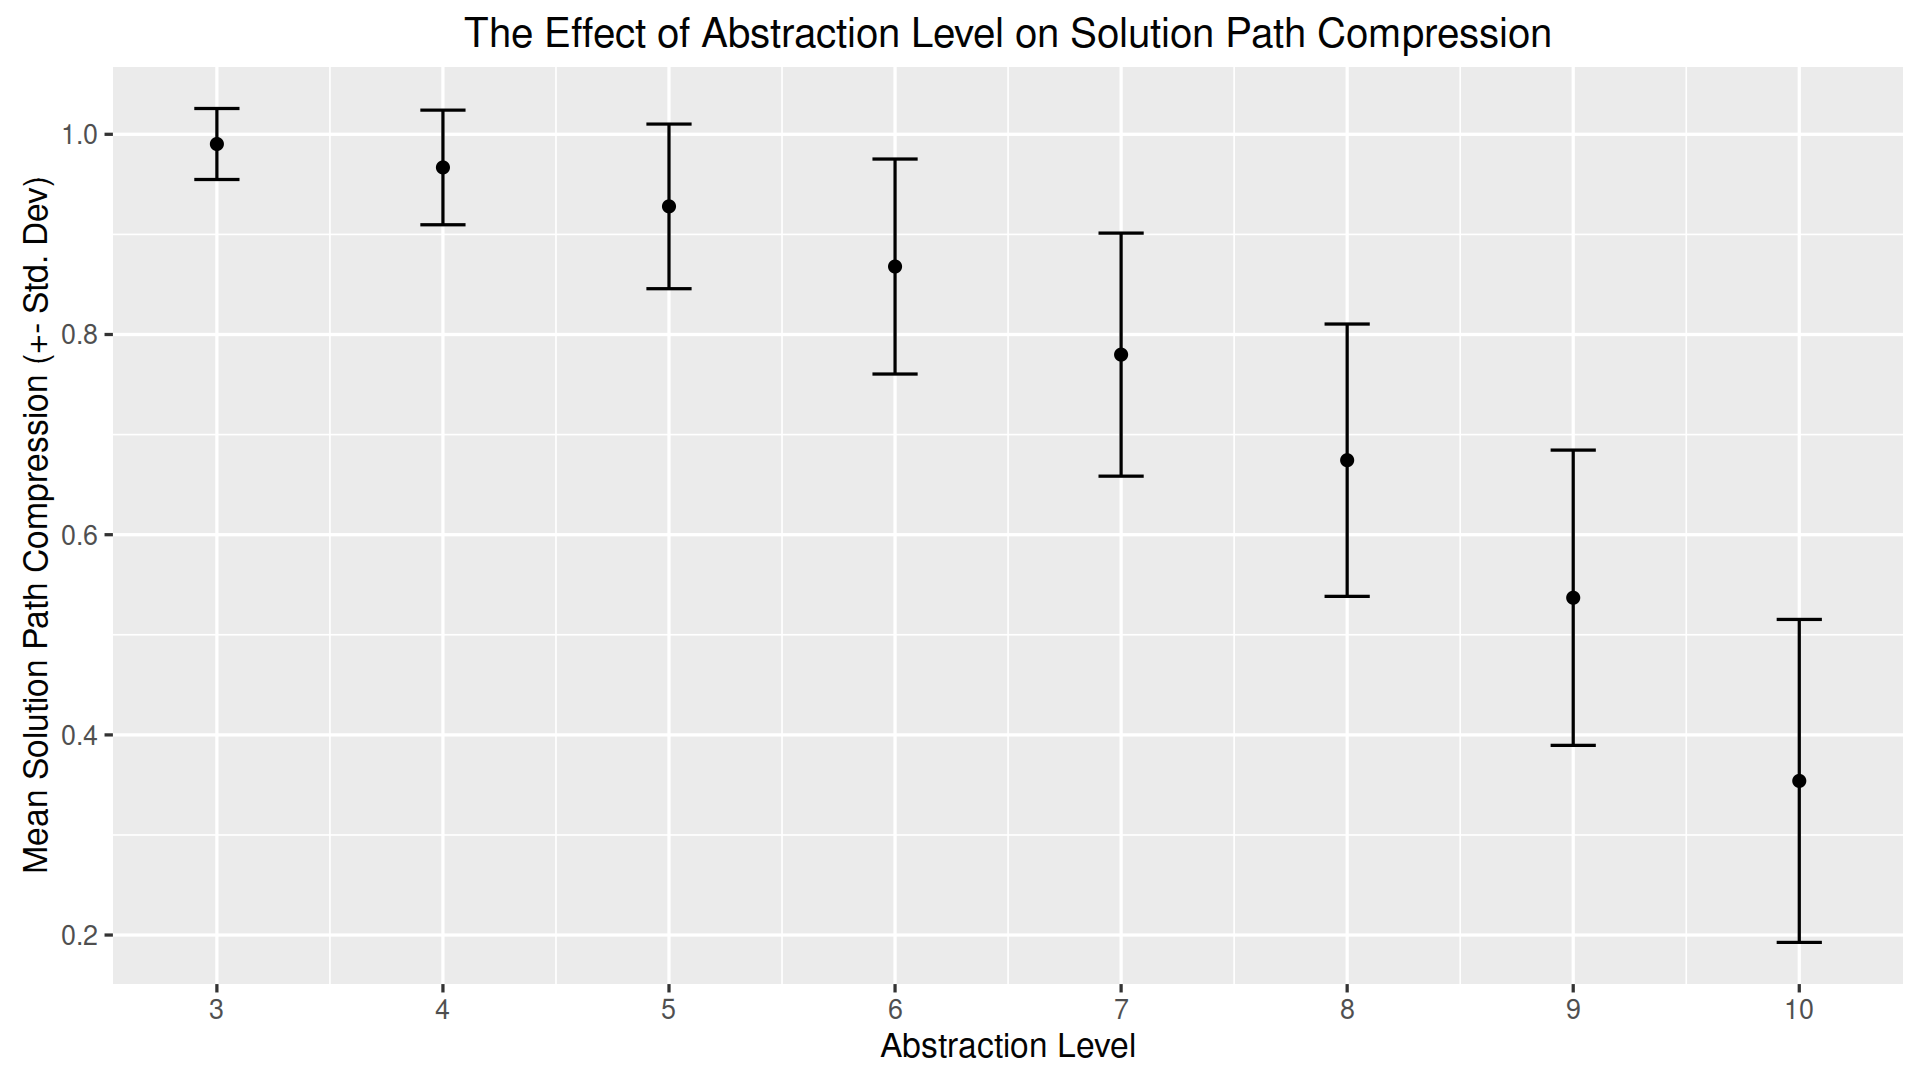
\includegraphics[width=1\textwidth]{path_compression_plot}
  \caption{Solution Path Compression in the Abstract Space}
  \label{fig:spc}
\end{figure}


We observe that the solution path becomes more compressed as we increase
the level of abstraction. This is not surprising; it is a result of the
increased State-Space Compression given by a higher level of abstraction.
For a given abstraction function \(a\),
and abstract initial and goal states, \(a(s_0)\) and \(a(s_g) \),
we have two sets of actual states, \(X\) and \(Y\),
that are  mapped to the abstract states:
\[\forall (x, y) \in X \times Y \text{, } \]
\[(a(x), a(y)) = (a(s_0), a(s_g))\]
Our domain abstractions produce an admissable heuristic,
meaning that if \(h(s, s')\) gives the cost of the optimal path from state
\(s\) to state \(s'\), we have \(h(a(s_0), a(s_g)) \leq min_{(x,y) \in X \times Y} (h(x, y))\).
Increasing the abstraction level also increases the number of states that are mapped to the same abstract state,
which increases the size of \(X\) and \(Y\),
and so \(h(a(s_0), a(s_g))\) will probably decrease. This would result in more Solution Path compression,
and thus the trend that we observe.\\

As a complimentary explanation for the observed results, suppose that our optimal solution in the unabstracted space is composed of a sequence of states \(s_0, s_1, \ldots, s_n = s_g\).
Then for our chosen abstraction, \(a\), we have \(a(s_0), a(s_1), \ldots, a(s_n)\) making up a valid abstract solution.
But if there are two states in the optimal solution,
\(s_i\) and \(s_j\), with \(0 \leq i < j \leq n\) such that \(a(s_i) = a(s_j)\),
then we could instead take \(a(s_0),\ldots,a(s_i),a(s_{j+1}),a(s_{j+2}),\ldots,a(s_n)\) as our solution
which is \(j - i\) states shorter. By the equivalence of \(a(s_i)\) and \(a(s_j)\) we note that
the transition \(a(s_i) \rightarrow a(s_{j+1})\) is a valid transition,
and so our shortened abstract solution remains valid.
Again, the likelihood of such a shortcut being found would be determined by the number of unabstracted states
which are represented by a single abstract state.
Therefore we claim that, as we increase the abstraction level,
the Solution Path Compression will probably increase. \\

Finally,
we observe that our two explanations for compression might
also cause a suboptimal unabstracted solution to be compressed so
that it becomes the optimal abstract solution. In any case,
the cost of optimal solution in the abstract space is less than
or equal to the cost of the optimal solution in the unabstracted space,
and as we abstract more tiles we expect to see more optimal solution cost compression.\\

We also notice that, for a given level of abstraction,
there is a variance in the path compression indicated by the standard deviation error bars.
This is merely a result of the fact that the path compression given by a level of abstraction is
influenced by the specific tiles that have been abstracted;
not all abstractions at the same level will produce the same path compression.
This makes sense when we consider that, for both of the explanations given above,
the path compression is not guaranteed to occur, it is just more likely as we increase the level of abstraction.
It could even be the case that a sampled abstraction produces no path compression at all.
We will see the effects of this variance in our further studies when we examine some
of values related to solution path compression. Notably, this will account for some of the variance
in our final predictions.

\subsubsection*{The Duplicate Probability Distributions for the Abstract Searches}

Our method of abstraction does not alter the Non-DSP branching factor of a node, which is determined solely by the
position of the blank (which remains unabstracted). Instead we claim that, for a given g-level,
increasing the level of abstraction increases the probability of nodes being
pruned as duplicates at that g-level, because we map some number of real nodes to abstract nodes.
In the real space, the paths to these nodes would not be terminated by DSP,
but if we trace these same paths in the abstract space, then we end up at the same abstract node,
resulting in each of those abstract paths being terminated by DSP.
In order to examine this behaviour,
for each abstraction level, we have plotted the mean duplicate probabilities at each g-level of
the abstract searches.
We have also plotted the duplicate probabilities at each \(g\)-level of the unabstracted search (abstraction level 0),
for comparison.
This graph is displayed in Figure \ref{fig:adpd}.
From these results, we are able to make a number of observations which support our hypothesis.
It should be noted that, for some abstraction levels,
we do not have a data point at every g-level.
This is a result of the solution path compressions that we observed earlier;
for those g-levels, all of the abstract searches happened to have found a solution at a shallower depth than the
actual solution cost. \\

\begin{figure}
  \centering
  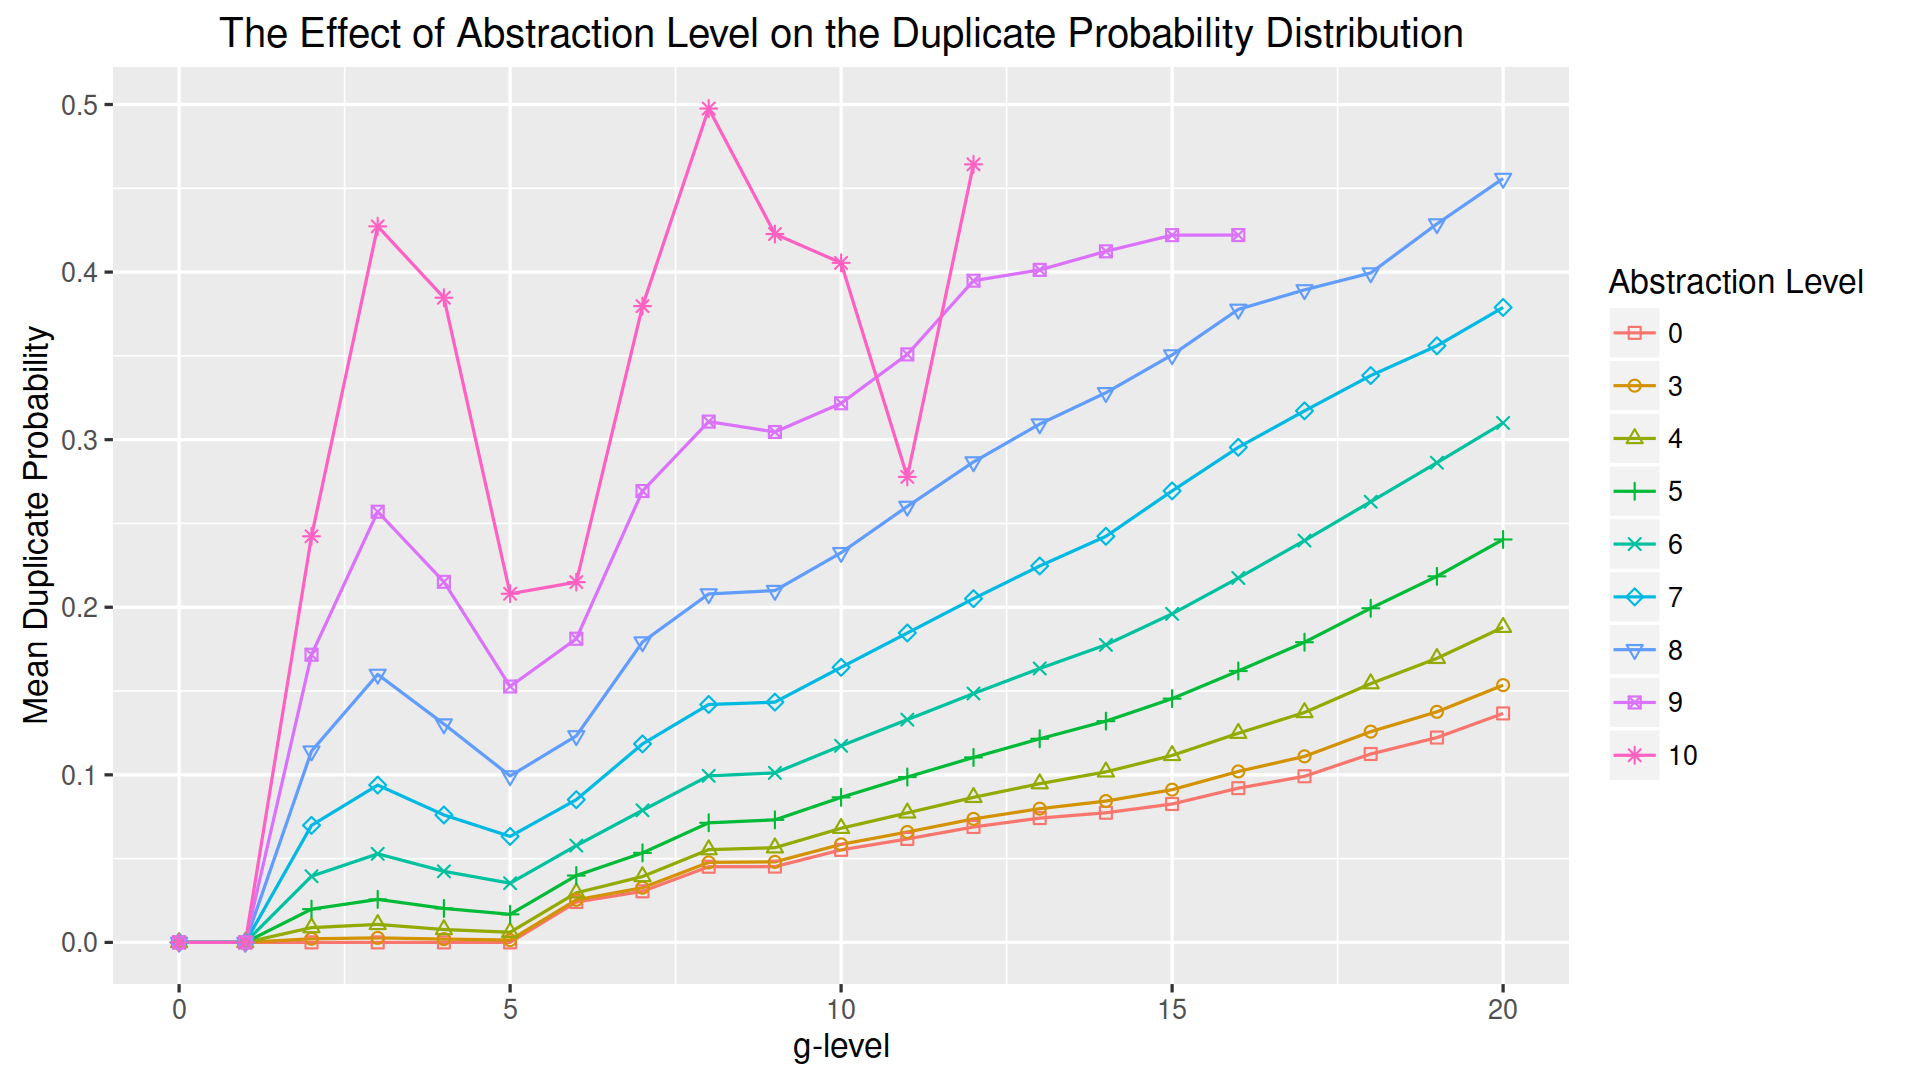
\includegraphics[width=1\textwidth]{g-level_vs_duplicates_plot}
  \caption{The Duplicate Probability Distributions for the Abstract Searches}
  \label{fig:adpd}
\end{figure}

We notice that (with some exceptions which we discuss below)
the duplicate probability tends to increase as the g-level of the search increases.
We assert that this correlation follows from the fact that,
as a search progresses, the total number of states that have been explored will increase.
A node is pruned as a duplicate only if it has already been explored before,
so as the g-level increases, you will have a larger number of stored states of
which a newly generated state may be a duplicate.
Suppose that we have run a search up to a given point, and we have generated some node, \(n\),
which represents a state, \(s(n)\).
Let \(explored(n)\) give the set of states that have already been explored by the search prior to expanding \(n\)
(i.e. the closed list),
and let \(reachable\) give the set of states that are reachable from the initial state.
We can see that \(n\) will be pruned as a duplicate iff \(s(n) \in explored(n)\).
If we were to assume that generating \(n\)
was the same as uniformly drawing \(s(n)\) from \(reachable\),
we would observe that
\[Pr(s(n) \in explored(n))) = \frac{|explored(n)|}{|reachable|}\]
We do not claim that this assumption is absolutely correct,
but it points to a positive correlation between \(\frac{|explored(n)|}{|reachable|}\) and \(Pr(s(n) \in explored(n)))\),
and so it stands as reasonable explanation as to the general trend that we observe.
Later on, we will examine the actual nature of this relationship in our searches. \\

Perhaps the most suprising feature of the plot is that the distributions
seem to follow a similar shape and curvature which is independant of
the Path Compression Factor. For each of the abstraction levels,
we observe some oscillations in the duplicate probability,
with spikes at g-levels 3 and 8,
and drops around g-levels 5 and 9.
We claim that this oscillation can be explained by distribution of blank types at each g-level of the search.
We note that a state and its duplicates all have the same blank type,
and thus we adapt our above explanation relating duplicate probability to explored states
so that it accounts for the probability of a node being a duplicate given that it
is of a specific blank type (recall that the blank type does not include information about the g-level or the parent,
only the position of the blank).
Suppose that we have run a search up to a given point, and we have generated some node, \(n\),
that we would like to know the duplicate probability for.
Let \(explored(n, t)\) give the set of states of blank type \(t\) that have already been explored by the search prior to expanding \(n\),
and let \(reachable(t)\) give the set of states of blank type \(t\) that are reachable from the initial state.
We can see that \(n\) will pruned as a duplicate iff \(s(n) \in explored(n, t)\).
If we were to assume that generating \(n\)
was the same as uniformly drawing a state from \(reachable(t)\),
we would observe that \[Pr(s(n) \in explored(n, t))) = \frac{|explored(n, t)|}{|reachable(t)|}\]
Again, this assumption is tenuous,
but it at least hints at how a node's type influences its duplicate probability.
It may be the case that for different \(t\),
we have \( \frac{|explored(n, t)|}{|reachable(t)|} \) growing at different rates.
This is particularly true early on in the search, where the type of the initial state
heavily influences the frequency of each type at shallower g-levels.
Korf et al. showed in their experiments that this is indeed the case \cite{korf2001time}.
Hence we would observe the duplicate probability fluctuating as the composition
of blank types changes for each g-level, and that this fluctuation would smoothen out as the g-level increases.
To complete our explanation,
we claim that the relative frequency of types at a given g-level is largely unaffected by the abstraction used,
and so the duplicate probability distributions exhibit oscillations at the same g-levels.
The basis for this claim comes from the observation that the type of a state and the types of its generated children will
remain unchanged after abstraction. Due to time constraints, we do not investigate this claim further. \\

We also notice that, as we hypothesised, for each g-level, the duplicate probability tends to increase as the abstraction level increases.
We consider two explanations for this observation.
First of all, we have already established that abstracting away more tiles
maps more unabstracted states to the same abstract state.
The abstract state is expanded once, corresponding to the shallowest of the unabstracted states
which are mapped to it.
Then whenever one of the deeper states would have been expanded in the unabstracted search,
that same path in the abstract space leads to a duplication of the abstract state.
So we would expect the probability of a node being pruned as a duplicate to be higher
in more abstract spaces, which is in line with the trend that we have observed.
Secondly, referring again to the relationship between the duplicate probability and proportion of the reachable state
space that has been explored, we have established that the size of \(reachable\) is compressed more as the abstraction level increases.
Assuming that the abstract \(explored\) is not compressed by that same amount for a given g-level in both the unabstracted and abstracted search,
we would necessarily observe a higher duplicate probability for that g-level.
Later, when we examine the relationship between \(explored\) and \(P\), we find some evidence which hints at this assumption
being the correct. \\

\subsubsection*{Search Tree Compression in the Abstract Space}

Ideally, we would like to be able to produce predictions quickly
enough that the time spent running our prediction algorithm is insignificant
compared to the actual search time.
We have proposed that we perform an abstract search in order to produce our predictions,
so we expect the runtime of our prediction to be highly dependant upon
the number of states expanded by the abstract search.
We may also consider the size of the abstract search trees
as a (somewhat poor) prediction for the size of the unabstracted tree.
Ultimately, we can compare these sizes to the predictions given by SSDP
in order to see how well our algoirthm compensates for the abstractions. \\

We have already examined the Solution Path Compression,
and the Duplicate Probabilities given by those abstract searches,
so we will now look at the effect that these results
have on the size of the abstract search trees.
We have recorded the number of abstract states expanded by each run of SSDP,
and then normalised these values as a proportion of the
number of nodes expanded during the actual unabstracted search.
We will refer to these proportions as the Search Tree Compression.
For each abstraction level, we summarise the Search Tree compressions for that level by taking the mean
compression
with error bars at
\(\pm\) 1 standard deviation about the mean.
We have plotted these values in Figure \ref{fig:stc}. \\

\begin{figure}
  \centering
  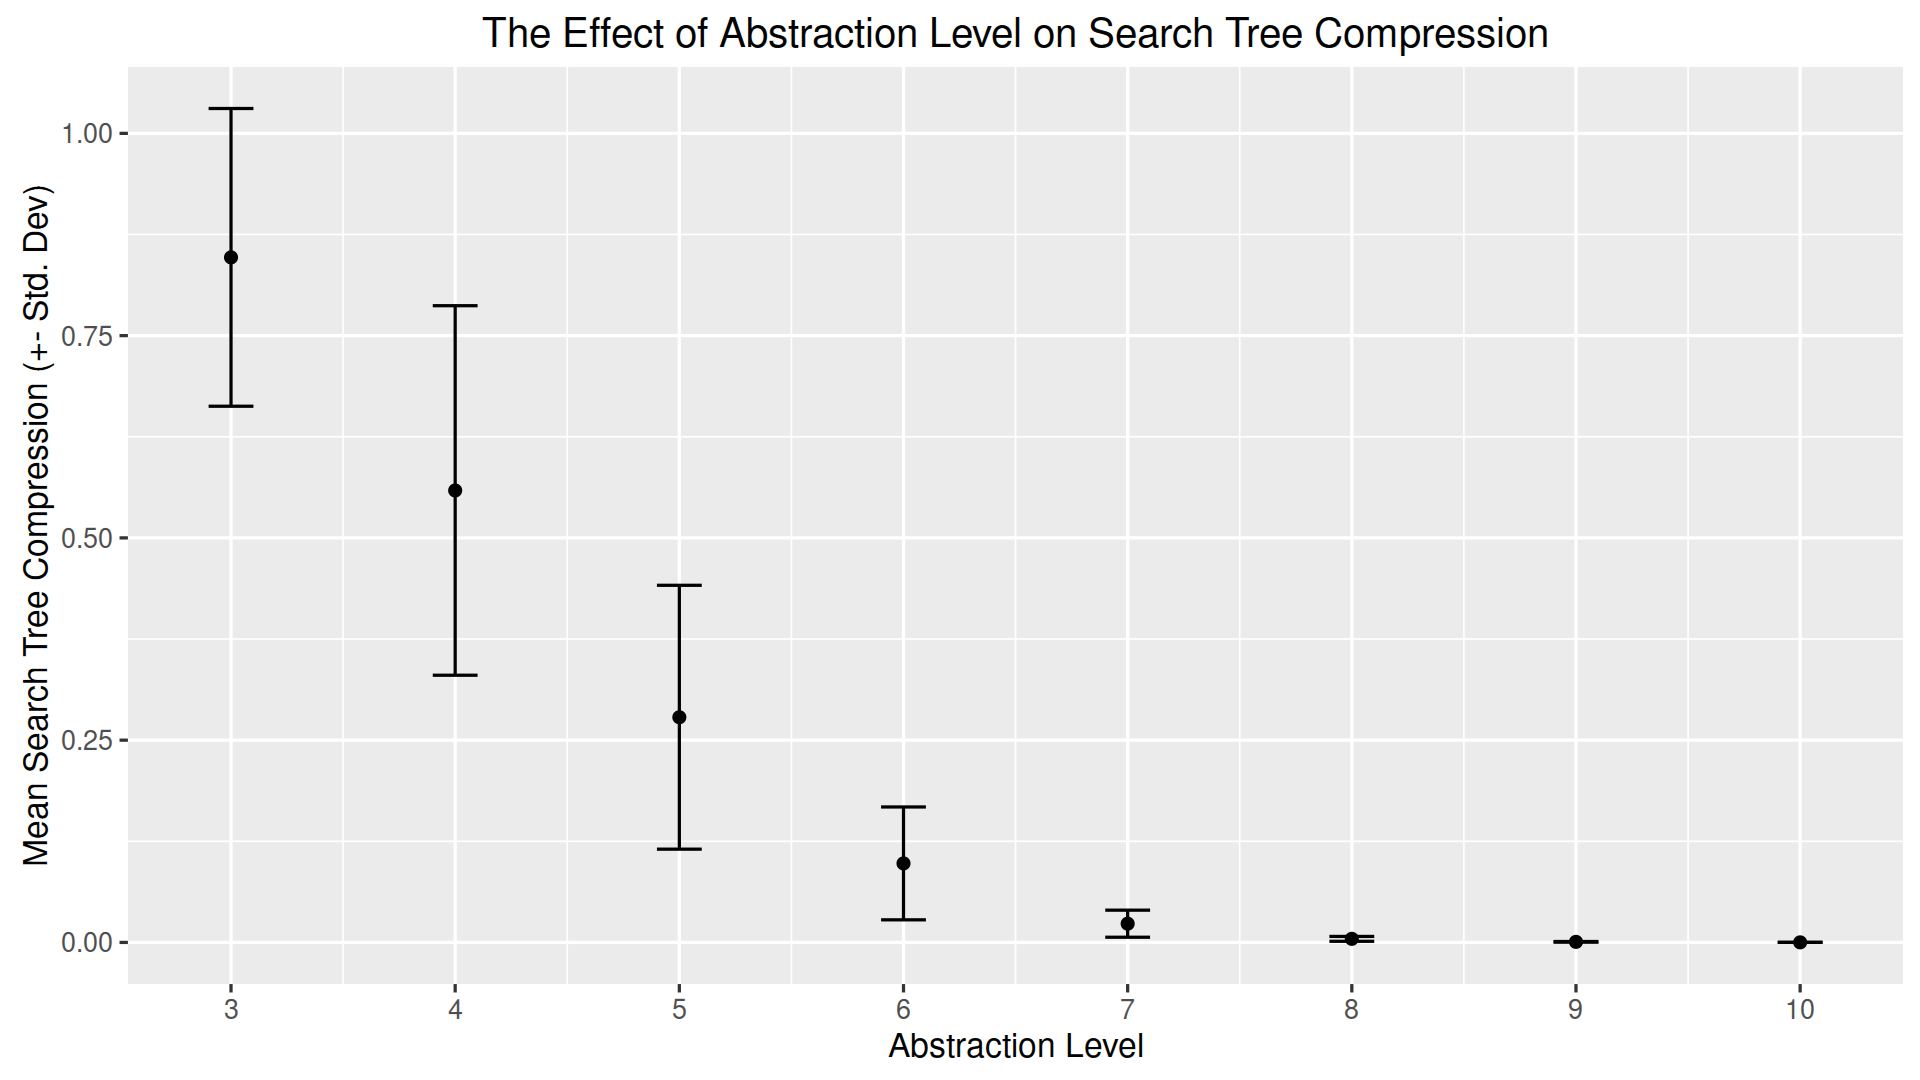
\includegraphics[width=1\textwidth]{search_tree_compression_plot}
  \caption{The Search Tree Compression in the Abstract Space}
  \label{fig:stc}
\end{figure}

As with the Solution Path Compressions,
we observe the Search Tree Compression factors trending downward
(i.e. more compressed) as the abstraction level increases.
We claim that this is a result of the effects of both the Solution Path Compression, and the Abstract Duplicate Probabilities.
Firstly, the Solution Path Compression will reduce the number of abstract states expanded because the
shorter solution path will result in a truncated search tree;
we don't expand nodes beyond the depth at which the abstract goal was found.
Secondly, the larger abstract Duplicate Probabilities reduce the branching factor of the abstract search tree
because we are using Duplicate State Pruning. The decreased branching factor will decrease the overall
size of the tree because, as we have shown before, the number of nodes at any given level of the tree is equal to the product
of the branching factors up to that level.


\subsection{Decompressing the Abstract Duplicate Probabilities}

We conclude from this work that in order to predict the behaviour of the unabstracted duplicate probabilities,
we must reverse the effect that state space compression has on the duplicate probability distribution.
Our problem is two-fold;
firstly, an abstract search does not give a duplicate probability at every depth of the search.
In order to account for this, we must somehow extrapolate our abstract results to deeper g-levels,
or transform our abstract results so that lower abstract g-levels map on to deeper unabstracted g-levels.
Secondly, we must account for the trend of duplicates probabilities being higher in abstracted searches for the same g-level.
We hypothesise that both of these problems can be solved by 'stretching' the abstract duplicate probability distributions by
their path compression factor.
Let \(P_a(t)\) give the proportion of generated type \(t\) nodes that were pruned as duplicates by abstraction \(a\),
and let \(C_a\) be \(a\)'s path compression.
Recall that our type system includes the \(g\)-level of a node as a part of its type.
So we construct our new type \(t_a\) to be the same as \(t\) except \(g(t_a) = g(t) \cdot C_a\).
Then we make our prediction for \(P(t)\), the unabstracted duplicate probability for type \(t\), as follows:
 \[P(t) \approx \hat{P}(t) = P_a(t_a)\]
 We are assuming here that the duplicate probabilities in the unabstracted search
 will map directly on to the duplicate probabilities in the abstracted search after compressing the g-levels
 by the path compression factor.
 Duplicate probability tends to increase both as \(g\)-level increases, and as abstraction level increases.
 In the unabstracted space,
 compressing the \(g\)-level would give us a decreased duplicate probability.
 But then taking the abstract probability at the compressed \(g\)-level will give rise to an increase.
 Our hope is that these two effects cancel eachother out, and the final value remains unchanged after
 the transformation.
 At the same time, this ensures that we take our predictions from \(g\)-levels that were explored by the abstract search:
 \[g(t) \leq h(s_0) \Rightarrow g(t_a) = g(t) \cdot C_a = g(t) \cdot \frac{h(a(s_0))}{h(s_0)} \leq h(a(s_0))\]. \\

 Unfortunately, we cannot simply retrieve \(P_a(t_a)\) from our abstract search results,
 because \(g(t_a) = g(t) \cdot C_a\) may not give a round number, whereas the \(g\)-levels of our abstract searches are discrete.
 Hence we construct \(t_{lower}\) and \(t_{upper}\) to be the same as \(t\) except that
 \(g(t_{lower}) = \lfloor  g(t_a) \rfloor\)
 and \(g(t_{upper}) = \lceil  g(t_a) \rceil\). We then interpolate between them to get our prediction:
 \[\hat{P}(t) =
   P_a(t_{lower}) + (g(t_a) - g(t_{lower})) \frac{P_{a}(t_{upper}) - P_{a}(t_{lower})}{g(t_{upper}) - g(t_{lower})}
 \]
 However, we are still not guaranteed that every type will occur at every level, hence
 for some \(t\) it might be the case that \(P_a(t_{lower})\) or \(P_a(t_{upper})\) are undefined.
 To handle these cases,
 if no nodes with type \(t_{x}\) were generated by our abstract search,
 then we take \(P_a(t_{x})\) to be the proportion of all nodes generated at \(g\)-level \(g(t_{x})\)
 that were pruned as duplicates by the abstract search (i.e. we ignore types altogether). \\

 
 If this method of prediction turns out to be accurate,
 we will be able to run an abstract search to find values for \(P_a\) and thus \(\hat{P}\).
 We can then supply \(\hat{P}\) to SSDP as our prediction for \(P\).
 The abstract searches will expand fewer nodes than the unabstracted search, and
 hence we achieve our goal of being able to predict the number of nodes expanded by the
 unabstracted DSP BFS search whilst doing less work than it would take to perform the search itself.


 
\subsubsection*{Our Predicted Duplicate Probabilities}

By the use of our pure type system,
we have shown that our predictions will be perfect when we are using the correct duplicate probabilities.
Therefore, in order to determine the cause for the errors in our final predictions,
we must first examine how well we are predicting those duplicate probabilities.
These predictions are produced via the decompression that we described in the previous section.
We used the same abstractions as we did in the previous experiment.
For each of the abstract searches,
we produced a prediction for the unabstracted duplicate probability distribution.
For each abstraction level, we have plotted the mean predicted duplicate probabilities at each g-level.
We have also plotted the actual unabstracted duplicate probabilities (abstraction level 0), for comparison.
This graph is displayed in Figure \ref{fig:pdpd}.
From these results, we can see how the abstraction level affects the accuracy of our duplicate predictions. \\

\begin{figure}
  \centering
  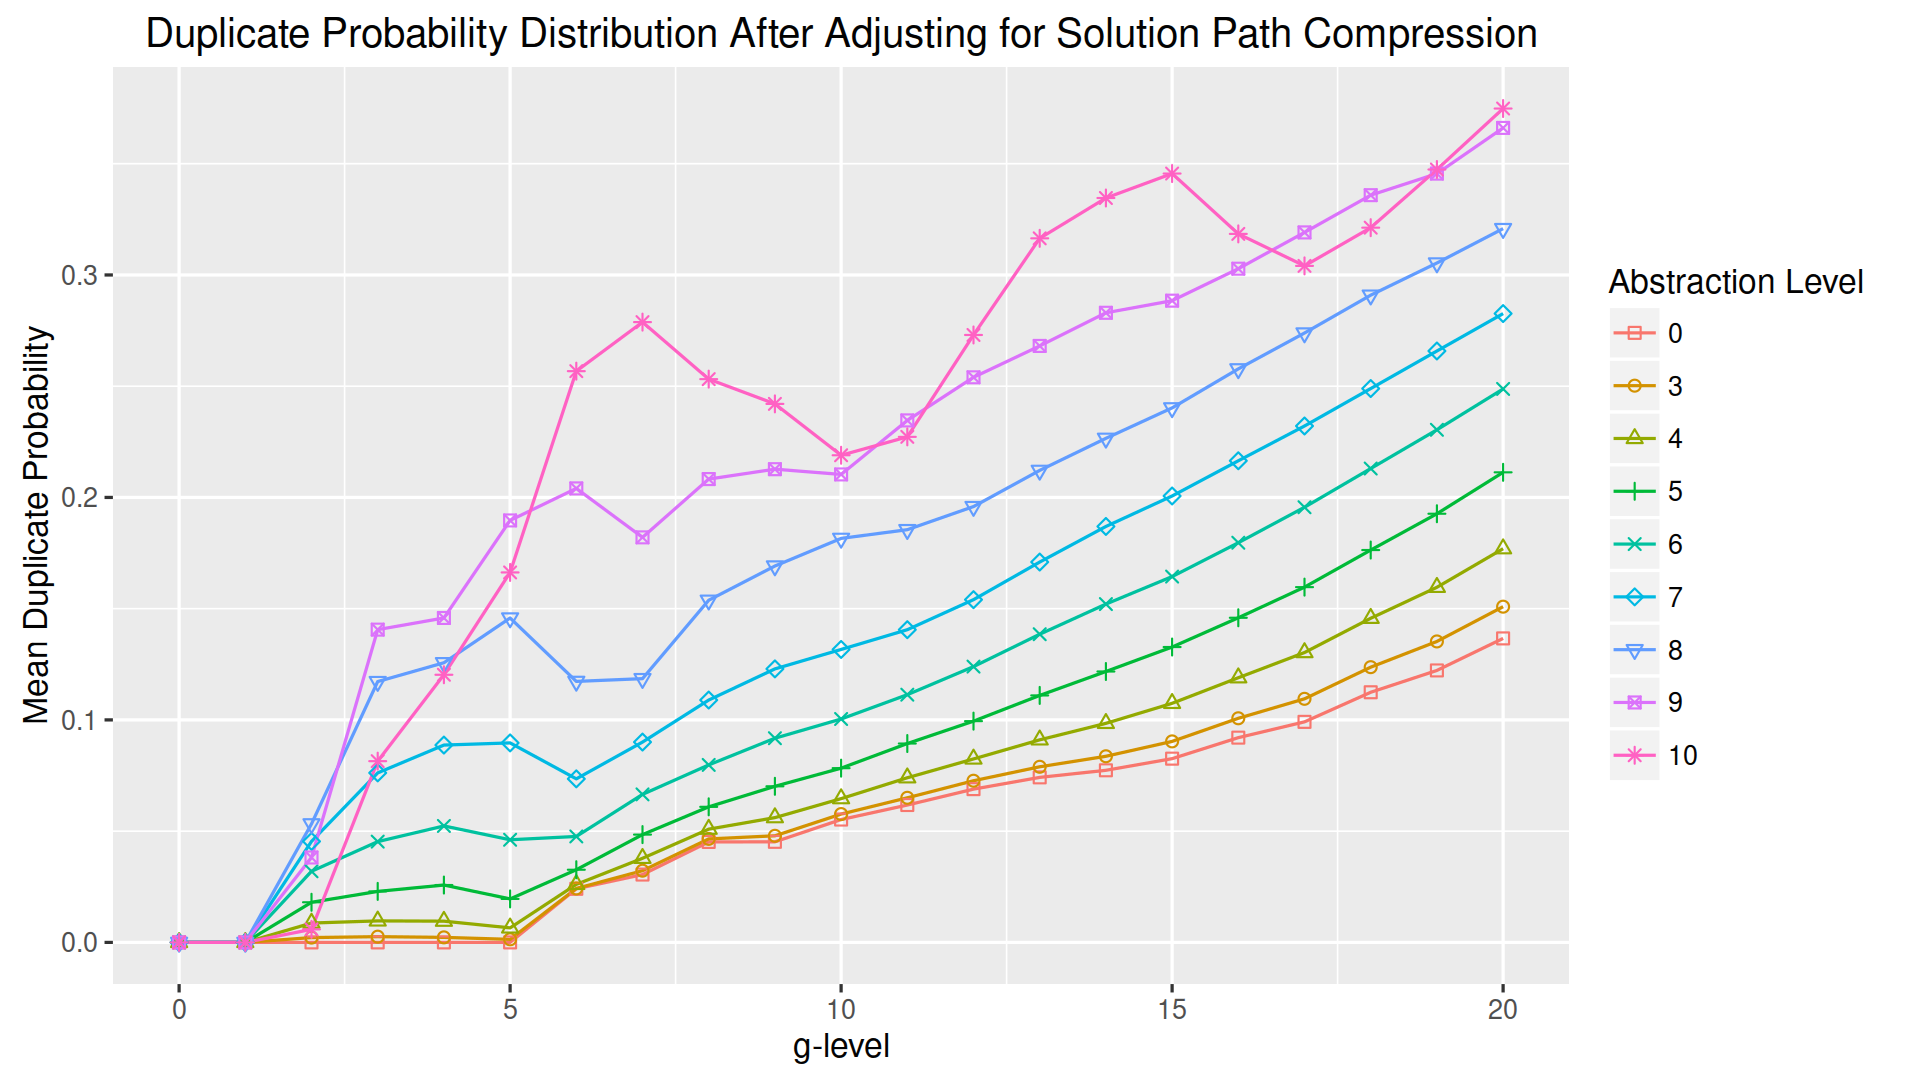
\includegraphics[width=1\textwidth]{pred_stats_plot}
  \caption{Our Predicted Duplicate Probability Distributions}
  \label{fig:pdpd}
\end{figure}

We draw attention to the fact that the predicted duplicate probabilities,
while not perfect, are something of an improvement over the unaltered abstract probabilities
in terms of approximating the actual values.
Our transformation allows us to obtain a prediction for the duplicate probability at every required \(g\)-level.
We also note that, going from the abstract results to the transformed results,
our path decompression scheme has had some effect in reducing the overestimation of the duplicate probabilities.
For example, at \(g\)-level 3, the mean value given by the unaltered \(10\)-tile abstractions was \(0.43\),
but after our transformation, we obtain a prediction of \(0.08\) which is closer to the true value of \(0.00\).
We observe that the transformed probabilities appear to be 'smoother' than their unaltered counterparts;
the oscillations are no longer as pronounced, and our maximum is now \(\leq 0.4\) rather than \(0.5\).
This is a result of our interpolation. The points along rapidly changing gradients are averaged,
and hence our peaks and valleys disappear.
This smoothing is appropriate when trying to predict the unabstracted probabilities, which are not as prone
to rapid direction change.
We also note that, for the lower abstraction levels like 3 and 4,
the predictions are quite accurate. This is probably because their
unaltered abstract probabilities were already quite close to the unabstracted value. \\

Unfortunately, we can also observe some worrying trends in our predictions.
Holding the \(g\)-level constant, as the abstraction level increases,
we can see that the predicted duplicate probability also increases.
This runs contrary to our assumption that the effects of the abstraction
would be counteracted by our \(g\)-level decompression scheme - if that were the case,
then we would expect to observe roughly equal duplicate probabilities for every level of abstraction.
Instead, it appears that the effect of the abstraction on increasing the duplicate probability
is greater than the effect of the path decompression on decreasing that probability.
This is an interesting result, we have not fully captured
the relationship between duplicate probability, abstraction level, and \(g\)-level.
It is apparent that the duplicate probabilities grow faster in the abstract space,
even when considered relative to the path compression factor.
This suggests that, if we were to try and improve this scheme, we would need to increase
the amount of \(g\)-level decompression that we apply.
But if the actual required decompression factor is not equal to the solution path decompression,
then we are met with the problem of deciding that proper decompression.
We can also see that the oscillations which were present in the original abstract results
are still present here, except they have been stretched so that they no longer
line up with the oscillations in the unabstracted results.
We saw that these features occurred at the same \(g\)-levels in the abstract results,
and so we should not have decompressed them. \\

Our results here show a bias toward overestimation
as abstraction level is increased.
This will negatively influence the accuracy of SSDP when we use the predicted \(\hat{P}\)
as input in to the algorithm.
We conclude that, if we were to improve this transformation scheme,
we must first figure out how to find the proper \(g\)-level decompressions.
We have found that these values are not equal to the solution path decompression,
and in fact they are larger than the solution path decompression.
We do, however, hypothesise that these values are related to the solution path decompression.
Though we do not test this claim here, we note that if this relationship exists,
and we were able to characterise it to give some transformation from solution path decompression
to the ideal decompression,
then we would be able to greatly improve the quality of our predictions.
An improved scheme also needs to account for the oscillations in the duplicate probability.
In our analysis of the abstract duplicate probabilities, we claimed that these oscillations
arose from fact that the relative frequencies of the state types at the early \(g\)-levels
remained largely unaffected by the abstraction. If this is the case,
then our transformation should also somehow weight duplicate probabilities according
to the frequency of those types.
It may also be the case that an entirely different prediction scheme is needed -
one that doesn't involve \(g\)-level decompression.
Referring again to our analysis of the abstract duplicate probabilities,
we claimed that there was some relationship between the proportion of the space
explored, and the duplicate probability.
We will examine this relationship later.

\subsubsection*{Using the Decompressed Duplicate Probabilities to Inform SSDP's Predictions}

Now that we have established the nature of the underlying abstract searches,
we can finally begin to examine the predictions that SSDP produces.
We will observe how our predictions for \(P\) alter our prediction of \(N_{DSP}\),
and attempt to explain the improvements of
our approach over the unadjusted abstract results.
We will also discuss the failings of our predictions
in relation to how our assumptions are supported and contradicted by the results. \\

For each of the abstractions from our experiment,
we have taken the duplicate probability and applied the path decompression.
Then with each of the predicted distributions \(\hat{P}\),
we ran SSDP with that distribution in order to produce a prediction \(\hat{N}_{DSP} \approx N_{DSP}\),
which estimates the number of nodes expanded by DSP BFS run on \(s_0\) up to depth \(h(s_0)\).
We have then normalised each of these predictions as a percentage of \(N_{DSP}\),
such that a perfect prediction would yield a value of \(1.0\).
Then we have plotted the abstraction levels against the mean normalised prediction
for that abstraction level, with error bars at \(\pm\) 1 standard deviation about the mean.
For comparison, we have also plotted the mean search tree compression for each abstraction level.
These values correspond to what proportion of the actual search tree size that we would have predicted,
had we simply taken the abstract search tree size as our predicted value. They also indicate
how long it took to generate those predictions.
The results are shown in Figure \ref{fig:ssdp}. \\

\begin{figure}
  \centering
  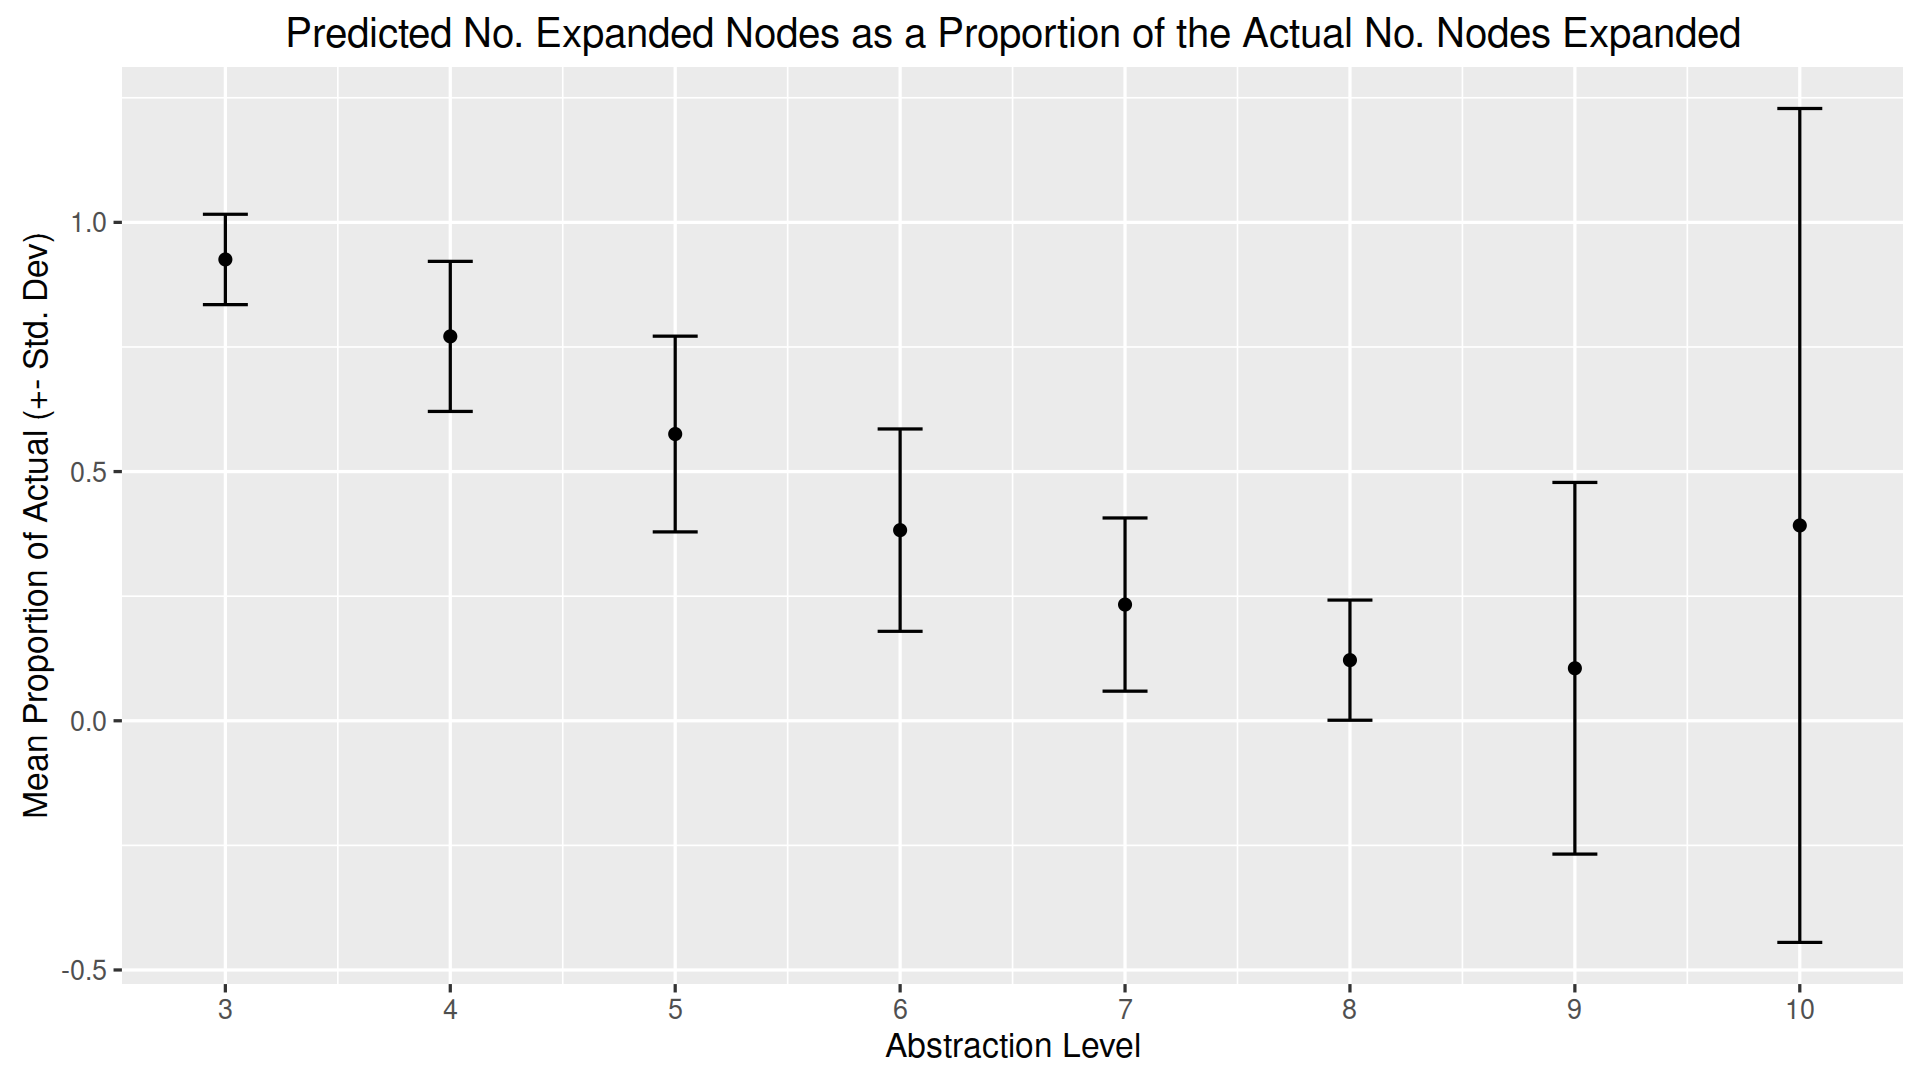
\includegraphics[width=1\textwidth]{predictions_plot}
  \caption{SSDP's Predictions}
  \label{fig:ssdp}
\end{figure}

Upon first observation, it is clear that these predictions are somewhat better than if we had just taken
the size of the abstract search trees as our predicted value. If we compare
these results to the search tree compression factors, we can see that our
use of path decompression, taken together with SSDP, has produced predictions
for \(N_{DSP}\) that are closer to the actual value.
In particular, abstraction levels \(3\) and \(4\) are producing excellent predictions.
This is to be expected, these abstractions do not compress the state space by very much,
and their duplicate probability predictions were quite close to the actual value.
The downside of the accuracy of their predictions is that we have still have to perform
a large amount of work to explore the abstract spaces which are not very compressed. \\

Unfortunately, we can see that there is a clear trend toward underprediction as the abstraction level increases.
This is clearly a result of the predicted duplicate probabilities being biased toward
overestimation as we increase the abstraction level.
SSDP weights its prediction for the number of type \(t\) nodes that were expanded by \(1 - \hat{P}(t)\).
Hence we observe an inverse relationship between the predicted number of nodes expanded,
and the predicted duplicate probability values.
We can also see that the variance of our predictions is quite large for abstraction levels \(9\) and \(10\).
This is probably a result of the fact that there are only a few abstractions at those levels,
and that the abstract state spaces are so granular that for some abstract searches,
we will by chance generate lots of duplicates,
and in others we won't generated any duplicates at all.
We should clarify that, though the error bars dip below \(0\),
this is actually just a result of the predictions being distributed unevenly about the mean -
our prediction scheme does not allow for a negative valued prediction. \\

Recall that we designed our SSDP algorithm and type system with the explicit intension of
removing all sources of error that didn't arise from our predictions of the duplicate probability distribution.
With a perfect prediction for the duplicate probabilities, we would have produced a perfect prediction
for \(N_{DSP}\). Thus we may conclude that all of the error that we observe in our predictions
arises only because our predictions for the duplicate probabilities are not correct.
It is therefore clear that, if we wanted to improve our \(N_{DSP}\) predictions,
we must improve our scheme for predicting the duplicate probabilities.
To that end, we will now investigate a possible alternative method for finding these probabilities.

\subsection{Using the Proportion of the Space Explored as a Predictor for Duplicate Probability}

It is now clear that we require a different approach to predicting the duplicate probability distributions.
During our investigation of the behaviour of the duplicate probabilities in the abstract space,
we claimed that, during the search, there was probably some relationship between the number of nodes explored and
the probability of a newly generated node being a duplicate. Specifically,
we claimed that if \(explored(n)\) gave the set of nodes that had been expanded prior to generating \(n\),
and \(reachable\) gave the set of states that were reachable from \(s_0\),
then the probability that \(n\) would be pruned as a duplicate was as follows:
\[Pr(s(n) \in explored(n)) = \frac{|explored(n)|}{|reachable|} \]
The basis for this claim came from the assumption that the generating \(n\)
was somehow similar to drawing \(n\) from \(reachable\) uniformly at random.
Obviously, this is not necessarily the case.
However, we do claim that there is some relationship between these two values.
Then let \(E(i) = \frac{\sum_{j = 0}^n N_{ex}(i)}{|reachable|}\) give the proportion of the space that we have explored up to level \(i\) of our DSP BFS search,
and let \(P(i)\) give the proportion of duplicates at level \(i\) of the same search.
We claim that there is some function \(R\) which captures the relationship between \(E(i)\) and \(P(i+1)\)
such that
\[R(E(i)) = P(i+1)\]
Suppose then that we know \(R\) and \(N_{ex}(i)\) for all \(i \leq j\),
and thus \(E(j)\). Recall our formula for \(N_{ex}\) and note that we can now substitute in \(R(E(j))\) for \(P(j+1)\):
\[N_{ex}(j+1) = N_{ex}(j) \cdot b_j \cdot (1 - P(j+1)) = N_{ex}(j) \cdot b_j \cdot (1 - R(E(j)))\]
Inductively, we can solve for any \(N_{ex}(i)\) as long as we know the branching factors and the size of the reachable space.
We are thus motivated to try and model the \(R\) relation.

\subsubsection*{Examining the \(R\) Relation for the Abstract Searches}

In our work, we will not go as far as using \(R\) as a predictive tool.
Rather, we have done some exploratory research examining how \(R\) behaves in the abstract searches.
Our aim is to motivate some future research, where we use the models of \(R\) given by the abstract searches
to model \(R\) in the real search. We hypothesise that this relationship is invariant of abstraction level,
because we account for the state space compression by dividing the number of nodes expanded by the size
of the reachable space for that abstraction. So for abstraction level \(x\),
we take \(E_x(i) = \frac{\sum_{j = 0}^n N_{ex}(i)}{|reachable(x)|}\) where \(|reachable(x)|\) is the size of the reachable state space
when using an \(x\)-tile abstraction.
Thus for each abstraction level \(x\), for each \(g\)-level \(i\) of the abstract searches at that abstraction level, we have plotted the mean \(E_x(i)\) against the mean \(P_x(i+1)\).
The results are shown in Figure \ref{fig:epdp}.
Please note that due to the exponential growth which is typical of BFS, it was required that the \(E_x\) values be plotted on a logarithmic scale. \\

\begin{figure}
  \centering
  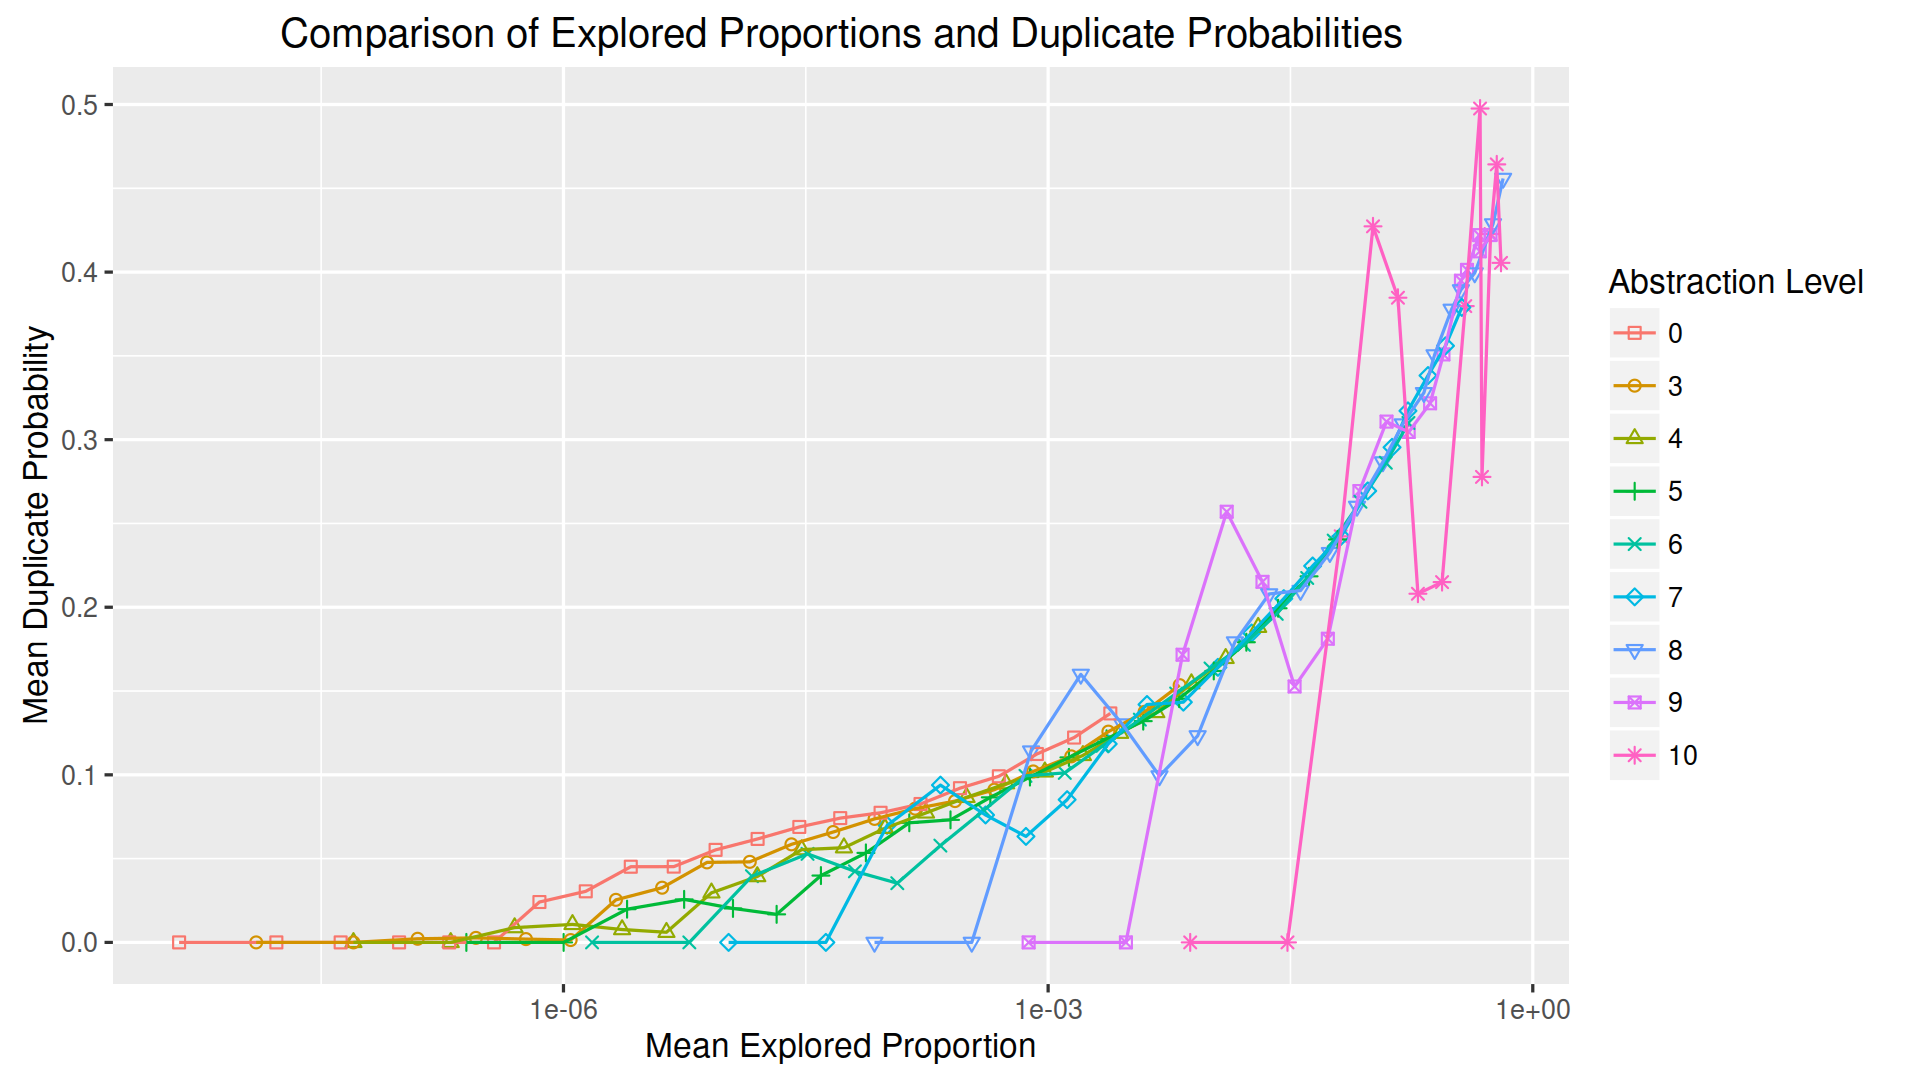
\includegraphics[width=1\textwidth]{explored_vs_duplicates_plot}
  \caption{The \(R\) Relation for the Abstract Searches}
  \label{fig:epdp}
\end{figure}


These results are very promising. We can see that, as we hypothesised, the \(R\) relation follows
the roughly same curve regardless of abstraction.
We note that, for a given level of abstraction \(x\), the smallest \(E_x\) value corresponds
to the proportion of the \(x\)-tile abstracted state space that we have explored when we have only explored the initial state.
This is why the plots start at a later \(E_x\) value when our abstraction level is higher.
The curve for each of the abstraction levels exhibits an initial oscillation.
As with the original abstract duplicate probability plot, we maintain that this occurs at the early \(g\)-levels
of the searches due to the relative frequencies of each type.
It may be the case that if we stratified our \(R\) relations by type, then the resulting curves would be smoother.
We can also see that, for an abstraction level \(x\), the largest \(E_x\) value increases as we increase \(x\).
This means that our abstract searches are exploring more of their reachable search space
than the unabstracted search. This would explain why we observed that,
by the end of our abstract searches, the duplicate probabilities were higher than the duplicate probabilities
at the end of the unabstracted search. This is partly what caused our \(g\)-level decompression to produce inaccuracies. \\

We conclude that the \(R\) relation is, for the most part, invariant when we change the abstraction level.
This suggests that we could indeed use the abstract searches to predict \(R\) and thus \(P\).
Hence we have found an alternative to our path decompression scheme, which may produce
more accurate predictions. More research is needed to confirm whether or not this is true.
The uniform nature of the \(R\) relation hints at existence of a formula which defines \(P\) in terms of \(E\).
Perhaps another option could be to attempt to discover this formula, and characterise the \(R\) relationship
more formally. Then we wouldn't need to perform the abstract searches at all.

\section{Conclusion}

The problem of predicting the number of nodes expanded by Non-DSP search has been addressed by a number of
researchers \cite{knuth1975estimating, purdom1978tree, chen1992heuristic, korf2001time, zahavi2010predicting, lelis2013predicting}.
They have provided a number of useful techniques such as branching factor sampling \cite{knuth1975estimating, purdom1978tree},
distribution based predictions like KRE and CDP \cite{korf2001time, zahavi2010predicting, lelis2013predicting},
and the hybrid approach SS \cite{chen1992heuristic}, which combines the idea of sampling with the use of a type system.
However, we have also observed that there has been very little research done in predicting DSP search,
with the only contribution in this area being SSDD \cite{lelis2014estimating}. We have proposed
an alternative algorithm, SSDP, which predicts the number of nodes expanded by DSP BFS search.
SSDP mimics SS except that it accounts for Duplicate State Pruning by multiplying the
representative weights by the proportion of nodes of that type that we expect will not be duplicates.
We showed that, given a pure type system and perfect knowledge of the duplicate proportion for each type of node,
SSDP would produce perfect predictions for the number of nodes expanded by DSP BFS search. \\

We then hypothesised that this duplicate probability distribution could be estimated by running
DSP BFS searches in the abstract spaces, as given via the application of domain abstractions to the original problem \cite{helmert2007flexible}.
In our experiments, we have examined the nature of the abstract duplicate probabilities over each of the \(g\)-levels of searches
for an \(11\)-Puzzle problem.
From our results, we conclude that we may be able to transform an abstract duplicate probability distribution in to an
estimation for the actual distribution by decompressing the \(g\)-values relative to the solution path compression factor
for that abstraction.
We have given a method for performing this decompression, and then applied it to each of our abstract duplicate probability
distributions in order to generate predictions for the actual duplicate probability distribution.
Our results showed that our predictions got worse as we increased the number of tiles used to produce the abstraction,
and that our decompression scheme was not completely accounting for the increased duplicate probabilities in the abstract searches.
Specifically, for the same \(g\)-level, increasing the abstraction level was correlated with an increase in the predicted duplicate probability
at that \(g\)-level.
Nevertheless, we observe that the predicted distributions were closer to the actual distribution
than if we had just used the abstract duplicate probabilities. \\

We have then supplied these predicted distributions as inputs to our SSDP algorithm.
The results showed that, as the abstraction level increased, the predictions given by the abstraction
would tend to underestimate the actual number of nodes expanded by the unabstracted BFS DSP search.
We concluded that this was a direct result of the overprediction for duplicate probability.
It was made clear that a better method of duplicate probability prediction was needed.
To that end, we proposed that rather than predicting the relationship between \(g\)-level and duplicate probability,
a better approach might be to predict the relationship between the proportion of the reachable space explored
and the duplicate probability. We hypothesised that this relationship was independant of abstraction level,
and thus the abstract searches could be used give estimations.
We used our experiment data to produce a preliminary analysis for
the viability of this method. Our results confirmed our hypothesis; the datapoints appeared to all fall along
the same curve regardless of abstraction. Hence we conclude that this is a promising approach.

\subsection{Future Research}
Our experimentation has made clear that our contributions leave some room for improvement.
In addressing the issue of predicting the number of nodes expanded by BFS with Duplicate State Pruning, we derived a method of prediction which relied on estimating the proportion of nodes that would be pruned as duplicates at each \(g\)-level of the DSP search. From our experiments,
we determined that a better method of producing these duplicate probability predictions was needed. From our preliminary results, modeling the relationship between the proportion of the space explored and the duplicate probabilities seems to be a more promising approach. Our immediate recommendation for future research is that we test how well these predictions perform when we use them to inform SSDP. \\

We note that our experiments were done with the \(11\)-Puzzle, with a single randomly generated initial state. It would be interesting to test our predictions on different problem instances, and with different problem domains. In particular, we supplied SSDP with a pure type system which gave perfect predictions for the branching factors. The SS framework is general enough to allow for impure type systems, with the guarantee that the branching factor predictions will at least be unbiased. The use of an impure type system may have some surprising results for our predictions of the duplicate probabilities.
We have also only considered uniform cost domains. Variable cost operators introduce some new complexities that need to be considered.when we generate our predictions. It is not obvious whether or not our method of predicting the duplicate probabilities will be robust to this change. \\

Our methodology only considered a very restricted class of abstraction, where we simply relabel tiles. It would be interesting to examine the behaviuor of the abstract searches when we introduce other methods of abstraction. For example, we could replace tiles with another blank space, and hence increase the number of possible tile sliding operations that are applicable to the abstract state. One immediately notices that this would alter the branching factors for the abstract states. This may have unforeseen consequences for our predictions. This perhaps suggests that some kinds of abstraction are better than others when using them to predict the behaviour of the unabstracted search. \\

Finally, we believe that a comparison should be made between our SSDP and the SSDD algorithm. Both of these predictive methods build upon the SS algorithm, and both of them aim to predict the number of nodes expanded by search which uses Duplicate State Pruning. Although we have mostly discussed SSDP in the context of predicting the nodes expanded by DSP BFS, it is also true that we have retained the functionality present in SS that allows us to predict the behaviour of A*. We therefore suggest that an experiment should be carried out which compares and contrasts the performance of SSDP and SSDD when predicting DSP A*.

\bibliography{dissertation}{}
\bibliographystyle{IEEEtran}

\end{document}
